\documentclass[12pt, a4paper, openany]{report}
\usepackage[left=3cm,top=3cm, bottom=3cm, right=4cm]{geometry}

% my custom stlye and functions stuff
\usepackage{mystyle}
\usepackage{csquotes}

\usepackage{setspace}

\pagestyle{fancy}
\fancyhf{}
\lhead{Jan van Dick}
\chead{\glqq Zweite Natur und Befreiung\grqq}
\rhead{\thepage}

\title{
    {\textbf{Zwischen Kritik und Affirmation}}\\ 
    {\large \color{darkgray}{Zweite Natur und Befreiung bei Hegel und Nietzsche}}\\
    {\bigskip}
    {\textbf{Between Critique and Affirmation}}\\
    {\large \color{darkgray}{Second Natur and Liberation in the Philosophies of Hegel and Nietzsche}}\\
    {\bigskip}
    {\large Goethe Universität Frankfurt am Main}\\
    {\bigskip}    
    {\bigskip}
    {\bigskip}    
    {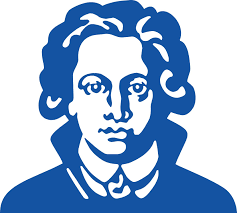
\includegraphics{logo.png}}\\
    {\bigskip}    
    {Sommersemester 2020}\\
}
\author{
    {Jan van Dick}\\
    {6081227}
    {Betreuer:}\\
    {Dr. Jonas Heller}
}
\date{\today}

\begin{document}

\maketitle
\frontmatter

\chapter*{Abstrakt}
\todo[noline]{welche Stellen des Abstrakts können noch aufgenommen werden?}
Friedrich Nietzsches These vom Tode Gottes aus \textit{Die Fröhliche Wissenschaft}, dass \glqq wir\grqq{} ihn getötet haben, ist mehr als bloße Negativität. 
Müsste der Mensch nicht selbst Gott werden, um ihn getötet zu haben?.\footcite[Vgl.][481]{nietzsche_morgenrote_1999} 
Und der Mensch ist Gott dadurch geworden, dass er ihn \textit{geschaffen} hat, dadurch nur konnte er ihn töten. 
In dem Tod Gottes, liegt, dass Gott selbst vom Menschen gesetzt, dass er Schein ist, der sich gegen ihn verselbstständigte.
Gott ist somit geistiges Produkt des Menschen, in dem der Geist selbst wieder zur Natur sich verkehrte.
Der Tod Gottes ist die Befreiung daraus.
Der \glqq Tolle Mensch\grqq{} erklärt aber zugleich, dass nur die wenigsten von dieser Tat wissen. 
Für die Einen ist der Tod Gottes, eine untergegangene Sonne, die Befreiung also wieder eine In-Natur-Verkehrtheit.
Nur für uns \glqq geborene Räthselrather\grqq, die den Tod Gottes im vollen Umfang begreifen, ist er ein \glqq neues offenes Meer\grqq\footcite[][573]{nietzsche_morgenrote_1999}.
Ist nun der Tod Gottes, die Befreiung aus der von ihm gesetzten Natur, das unbekannte, neue, offene, noch nie so offen gewesene Meer, oder ist er der Beginn des Wieder-in-Natur-Verkehrt-Seins, wie Christoph Menke es in der Analyse Hegels Begriffs der zweiten Natur beschreibt?\footcite[Vgl.][144]{menke_autonomie_2018}\\
Befreiung steht also zwischen Kritik (wieder-in-Natur-Verkehrtheit) und Affirmation (Einheit von Setzen und Sein).
Während Menke (und Hegel) Befreiung aus der zweiten Natur, nicht ohne eine neu hervorgebrachte zweite Natur, in welcher der Geist wieder in Natur verfällt lesen, erörtere ich die Frage, ob es in dem Motiv des \glqq neuen offenen Meeres\grqq{} und der \glqq geborenen Räthselrather\grqq{} bei Nietzsche, eine Befreiung aus der fortwährenden In-Natur-Verkehrtheit geben kann.
Es ist die Frage nach einer dritten Befreiung neben der Befreiung aus der 1. und der 2. Natur. 
Die Antwort dazu wird sich in der Arbeit als Ergebnis des Unterschiedes der \glqq Erkennenden\grqq{} bei Nietzsche geben:
Zwar kann Befreiung aus der Natur nicht ohne Setzen einer zweiten Natur geschehen, aber die Befreiung, die sich in dem Bewusstsein ihrer eigenen Kritik vollzieht, ist zugleich über ihrer eigene Befreiung hinaus.
Die dritte Befreiung ist damit allerdings keine Befreiung aus der Befreiung.
Befreiung bleibt notwendig: der Mensch kann Freiheit nicht \textit{haben}, er muss sie immer wieder selbst hervorbringen.

\onehalfspacing
\tableofcontents

\mainmatter

\chapter{Einleitung}
So, wie Friedrich Nietzsche in dem Aphorismus vom \glqq Tollen Menschen\grqq{} in \textit{Die fröhliche Wissenschaft} die These vom Tode Gottes entfaltet, enthält sie weit mehr als die bloße Negation Gottes;
in ihr steckt eine dialektische Konzeption der Begriffe (zweite) Natur und Befreiung.\footcite[Vgl.][481]{nietzsche_morgenrote_1999}
Diese beiden Begriffe möchte ich aus der Sicht Nietzsches, sowie der von Christoph Menke rekonstruierten Perspektive Hegels untersuchen.
Beide Begriffe entfalten sich in ihrem Doppelcharakter: zweite Natur als Kritik und Affirmation, Befreiung als Macht und Ohnmacht des Geistes.
In der zweiten Natur schlägt Setzen in Sein um; hierin liegt zum Einen die Verwirklichung des Geistes (Affirmation), zum Anderen die In-Natur-Verkehrtheit, der Tod des Geistes durch den Geist (Kritik).\footcite[Vgl.][145]{menke_autonomie_2018}
Ebenso verhält es sich mit dem Begriff der Befreiung: 
sie ist 1. die \textit{Macht} des Geistes neues Hervorzubringen und die scheinbare Notwendigkeit des Bestehenden zu durchbrechen, 
2. aber die \textit{Ohnmacht} des Geistes, da die Befreiung nie abgeschlossen ist; die Macht der Befreiung ist die Schaffung einer \glqq neuen\grqq{} zweiten Natur, aus der der Geist sich befreite und nun erneut befreien muss.\footcite[Vgl.][80]{menke_autonomie_2018}\\
Doch während in Hegels Deutung der Geist in der Befreiung aus der zweiten Natur, auf Grund der Endlichkeit des menschlichen Geistes, wieder in Natur verfällt, scheint bei Nietzsche in der Metapher des neuen, offenen Meeres, die Perspektive die ewige Wiederholung der In-Natur-Verkehrtheit zu überwinden, gegeben zu sein.
Zugleich betonen sowohl Hegel, als auch Nietzsche Freiheit als nicht-gegeben: 
Freiheit wird bei beiden so gedacht, dass man sie \glqq nicht nur hat, sondern auch beständig  noch erwirbt und erwerben muss\grqq\footcite[][637]{nietzsche_morgenrote_1999}. 
Freiheit ist die Befreiung aus der jeweiligen Unfreiheit.\footcite[Vgl][227]{adorno_negative_dialektik_2003}
Die Dialektik zwischen Freiheit und Notwendigkeit, Geist und Mechanismus, Endlichkeit und Unendlichkeit des Geistes, ist demnach Gegenstand meiner Arbeit. 
Die Leitfrage der Arbeit also: \textit{gibt es in Nietzsches Philosophie eine Möglichkeit der Überwindung der Notwendig-in-Natur-Verkehrtheit des Geistes?}\\
Aus der Position des oben erwähnten \glqq Tollen Menschen\grqq{} liegt es nahe, diese Möglichkeit in dem \textit{Vollzug} der Befreiung zu denken. 
Genauer: in einer Form des Bewusstseins in der Tätigkeit der Befreiung; 
eine Befreiung, die sich im Bewusstsein ihrer eigenen Kritik vollzieht.
Zugleich, muss aber der Schein selbst, \glqq mich fühlen lassen, dass hier Schein [...] und nichts mehr ist\grqq\footcite[][417.]{nietzsche_morgenrote_1999}.
Zu fragen wäre demnach, ob dieses Bewusst-Werden eine Arbeit des einzelnen Individuums ist, oder ob es aus der Struktur des Allgemeinen, aus der zweiten Natur, dem Schein selbst, hervorgehen kann.\\

Nietzsche Aussage über den Tod Gottes bedeutet nach der Form-Seite die Überwindung der vom Menschen gesetzten zweiten Natur (Gott), der inhaltlichen Seite nach aber, dass der Mensch Gott nicht mehr nötig hat und die Bestimmung des Gesetzes sich aus dem Menschen selbst entwickelt. 
Um also den Begriff der zweiten Natur zu erarbeiten, werde ich kurz auf den Begriff der Autonomie eingehen, da hier der Versuch, Gesetz und Freiheit zusammen und von Gott gelöst zu denken, seinen Ursprung nimmt. 
Der Begriff der zweiten Natur ergibt sich dann aus Hegels Kritik an Kants Autonomiebegriff.
%versucht Kant zwar mit dem kategorischen Imperativ aus dem Paradox der Autonomie zu entkommen, argumentiert Hegel, dass er sich hier in der Inhaltslosigkeit des Gesetzes wiederholt.
Hegels Ausweg besteht darin Freiheit sozial zu verstehen. 
Aus dieser Perspektive werde ich Hegels Begriff der Sittlichkeit als soziale Teilhabe entwickeln.
Doch hier wird sich das Paradox der Autonomie in dem Begriff der Gewohnheit wiederholen.
Aus der erneuten Wiederholung des Paradox werde ich Hegels Begriff der Befreiung entwickeln.
Darin ergibt sich, wie oben angegeben, die Grenze des von Menke erarbeiteten Begriffs der Befreiung:
Macht und Ohnmacht der Befreiung: Freiheit und Unfreiheit bleiben untrennbar miteinander verbunden.
Durch die Hinzunahme Nietzsches, soll versucht werden über diese Grenze hinauszugehen.\\

\todo[noline]{This part and the next seam to say more or less the same}
Zunächst soll der Begriff der zweiten Natur aus der Perspektive Hegels erläutert werden. 
In einem \hyperref[abschnitt_1]{ersten Schritt} soll demnach der Hegelsche Begriff der zweiten Natur anhand von folgendem Zitat Menkes rekonstruiert werden:
\begin{itemize}
    \item[] Die Gewohnheit als zweite Natur [ist] geistig oder frei [...], insofern sie ein Ausdruck des Wollens (oder ein Setzen) ist, und [...] mechanisch oder unfrei [...], weil sie, einmal gesetzt, selbstständig und unbewusst wirkend ist.\footcite[][145]{menke_autonomie_2018}
\end{itemize}
Die Struktur des ersten Teils ergibt sich aus den zu klärenden Begriffen. 
Zuerst soll der Begriff der Gewohnheit aus der Sittlichkeit, als Schritt über den \glqq bloß moralischen Standpunkt[]\grqq\footcite[][§ 135, S.139]{hegel_grundlinien_2017} hinaus, erläutert werden (a). 
Daraus ergibt sich der Begriff des \qq{geistigen Mechanismus}, in welchem die Gewohnheit sich als \qq{geistig oder frei} und \qq{mechanisch oder unfrei} ergibt (b).
Schließlich soll der Begriff der zweiten Natur aus Hegels Perspektive, seinen Abschluss finden in der Dialektik zwischen endlichem und unendlichem Geist und dem Doppelcharakter der zweiten Natur als Kritik und Affirmation (c).\\
In einem \hyperref[abschnitt_2]{zweiten Schritt} soll gezeigt werden, dass bei Nietzsche ein ähnlicher Begriff der zweiten Natur aufgezeigt werden kann.\footnote{Ich halte diesen Schritt unter anderem des deshalb für sinnvoll, weil er rechtfertigt, warum ich meine, mit Nietzsche überhaupt über Menkes Begriff der Befreiung hinausgehen zu können.}
Dabei soll bereits auf die Beantwortung der Leitfrage vorbereitet werden.
Zunächst soll der Begriff der zweiten Natur anhand von Nietzsches Begriff des \textit{Scheins} erläutert werden (a).
Die Befreiung aus dem (sog.) Schein wird darauffolgend in der Unterscheidung des Schauspielers und der Rolle aufgegriffen (b). 
Abschließend sollen beide Begriffe nochmals in dem Absatz über den tollen Menschen analysiert und zusammengebracht werden (c).
In der Darlegung Nietzsches Position wird der Begriff \glqq Bewusstsein der Scheinhaftigkeit\grqq{} bereits eine wichtige Rolle einnehmen und dient der späteren Beantwortung der Leitfrage.\\
Im \hyperref[abschnitt_3]{dritten Abschnitt} soll das Problem der Befreiung aus der zweiten Natur erläutert werden, da diese, im Vergleich zur Befreiung aus der ersten Natur bei Hegel und Menke, und letztendlich auch bei Nietzsche, uneindeutig bleibt.
%Wie Befreiung aus der zweiten Natur überhaupt möglich ist und wie diese sich konkret vollzieht, ist notwendig, um zu diskutieren wie über diese hinausgegangen werden kann.\\
Im vierten und \hyperref[abschnitt_4]{letzten Schritt} soll es abschließend zu einer Diskussion und Beantwortung der Leitfrage kommen. 


\chapter{Hauptteil}
Um nochmals einen anderen Einstieg zu wählen und die Fragestellung, sowie den groben Umriss der Arbeit auf alternative Art und Weise darzustellen, und die Problematik gewissermaßen von hinten aufzurollen, sei hier ein Zitat Nietzsches vorangestellt, auf welches ich gegen Ende erneut eingehen werde:
\begin{itemize}
    \item[] \textelp{} so finden wir als reifste Frucht an ihrem [der Sittlichkeit] Baum das \so{souveraine} [sic] \so{Individuum}, das nur sich selbst gleiche, das von der Sittlichkeit der Sitte wieder losgekommene, das autonome übersittliche Individuum (denn \qq{autonom} und \qq{sittlich} schliesst sich aus) \textelp{} \footcite[][293]{nietzsche_jenseits_2014}
\end{itemize} 
Hier befinden sich verschiedene Konzepte und Probleme im Begriff der Freiheit und im Geist-Natur-Verhältnis, die in der folgenden Arbeit eine zentrale Rolle spielen. 
Diese sollen als Einleitung der Auseinandersetzung mit den Begriffen \emph{Befreiung} und \emph{zweite Natur} vorangehen.\\

\emph{1. Geist als aus der Natur hervorgehend und sich von ihr unterscheidend.}\\
Zunächst spricht Nietzsche im selben Abschnitt von der Sittlichkeit als eine \qq{\so{vorhistorische} Arbeit}\footcite[][293]{nietzsche_jenseits_2014}.
Diese Sittlichkeit beschreibt Nietzsche als die Entwicklung des Menschen, in der er sich durch Zurichtung und Gewohnheit von seiner Natur befreit, die aber zugleich der Freiheit gegenübersteht, weil sie eine neue Form von inneren Zwang, von innerer Notwendigkeit schafft (\qq{der Mensch [muss] \textelp{} \emph{notwendig} geworden sein}\footcite[][292]{nietzsche_jenseits_2014}).
Darum ist die \qq{reifste Frucht} der Sittlichkeit dasjenige Individuum, welches sich von ihr wieder befreit.
Ohne hier den Anspruch zu erheben, Nietzsche habe es genau so gemeint, oder sei selber Hegelianer, liegt hier dennoch etwas vor, was stark an Hegels Begriff des Geistes erinnert, nämlich, dass er dadurch bestimmt ist \qq{aus der Natur herzukommen und sich von der Natur zu befreien}\footcite[][294]{khurana_freiheit_2017}.%
Dies bedeutet, dass der Geist nicht einmal aus der Natur hervorgegangen ist, sondern es immer wieder und immer wieder auch in den höheren Stufen des Geistes tut.
Wenn der Geist, wie Hegel sagt, wesentlich die Bewegung seiner Befreiung aus der Natur ist, dann ist die Frage, \emph{welche} Natur es ist, aus der er sich immer wieder befreit. 
Es ergibt sich daraus, dass der Geist selbst, durch diese Bestimmung, zur Natur zurückgeführt wird und, dass die Natur, aus der er sich befreit, letztendlich eine Natur ist, die er sich selbst voraussetzt: zweite Natur.\footcite[Vgl.][320]{khurana_freiheit_2017}
Das meint Nietzsches Rede vom Vorhistorischen: 
der Geist hat sich von der Natur befreit, indem er die Sittlichkeit, seine eigene (zweite) Natur gesetzt hat. 
Das Nicht-Mehr-Vorhistorische ist, sich auch von dieser wieder zu befreien.
Dadurch hat Freiheit auch bei Nietzsche explizit prozesshaften Charakter. 
Wie in der Einleitung bereits angedeutet, liegt hier auch die Leitfrage meiner Arbeit: \emph{inwiefern kann dieser Prozess aufhören und zu einem Ende kommen?}
Nietzsche spricht diesen Ausweg ganz konkret an, er spricht vom \qq{Ende des ungeheuren Prozesses} und vom \qq{übersittliche[n] Individuum}, welches an dessen Ende steht.\footcite[][293]{nietzsche_jenseits_2014} 
Aber ist dieses Ende auch bei Nietzsche schließlich so zu verstehen, dass kein Prozess mehr stattfindet und der übersittliche Menschen, seine Autonomie \emph{hat}?
Diese Frage soll am Ende der Arbeit beantwortet werden.\\

\emph{2. Sittlichkeit als Kontrast zur Autonomie}\\
Meine Arbeit wird von dem Begriff der Autonomie ausgehen. 
Hier werde ich zunächst das Paradox, in welches sich die Autonomie verstrickt und dann den Ausweg in der Sittlichkeit beschreiben.
Spannend ist, dass Nietzsche hier Autonomie als den Schritt über die Sittlichkeit \emph{hinaus} bestimmt:
Autonomie ist insofern der Anfang, und das Ende des Prozesses.
Dies ist darum so spannend, weil Nietzsche dennoch deutlich macht, dass die Sittlichkeit der notwendige Schritt \emph{vor} dem autonomen Individuum ist und zugleich schließt seine Sittlichkeitsdefinition an Hegels Kritik an Kants moralische Konzeption an.
Nietzsche definiert Sittlichkeit als \qq{die \emph{herkömmliche} Art zu handeln und abzuschätzen}.%
\footnote{
    \fullcite[][22]{nietzsche_morgenrote_1999}. 
    Nietzsche verweist im oben zitierten Abschnitt explizit auf diese Stelle der Morgenröte
    }.
Ebenso definiert auch Hegel die Sittlichkeit als handelnde Verwirklichung des Guten\footcite[Vgl.][§142, S. 161]{hegel_grundlinien_2017} und diese Definition, über das Handeln, bildet die Kritik an Kants formalistischer Definition.
Insofern kann gesagt werden, dass Nietzsche Hegels Kritik an Kants Autonomieformel zustimmt, und ebenso Sittlichkeit als den Schritt über die moralisch-autonome Form hinaus versteht, allerdings auch über die Sittlichkeit wieder hinaus will.
Die Autonomie muss, so könnte man sagen, \emph{durch die Sittlichkeit hindurch}.\\

\emph{3. Kritik: Freiheit als das sich Bestimmende}\\
Der dritte Aspekt deutet sich genau an dieser Stelle an. 
Während Kants formalistische Definition der Freiheit inhaltsleer bleibt, kann nach Hegel Freiheit nicht als reine Unbestimmtheit oder bloße Abstraktion verstanden werden.
Neben dem Moment der bloßen Unbestimmtheit, ist die einfachen Bestimmung gleichsam ungenügend, da sie \qq{eben so \emph{Negativität}, Aufheben [ist] als das erste - es ist nämlich das Aufheben der ersten abstrakten Negativität.}\footcite[][39]{hegel_grundlinien_2017}
Khurana drückt dies so aus, dass das Subjekt einer Bestimmung bedarf, die dem Ich einen konkreten Inhalt gibt und (diese Bestimmung) selbst die Form des Ich erhält\footcite[Vgl.][285]{khurana_freiheit_2017}. 
Freiheit ergibt sich erst in der Einheit dieser beiden Momente und Freiheit des Willens ist eben das: sich \qq{in Einem, sich als das Negative seiner selbst, nämlich als \textit{bestimmt}, \textit{beschränkt} zu setzen und bei sich, d.i. in seiner \textit{Identität} mit sich und Allgemeinheit zu bleiben.}\footcite[][40, §7]{hegel_grundlinien_2017}\\

\emph{4. Bei sich sein im Anderen}\\
Hieraus kommt Khurana auf Hegels Formel des \qq{Bei-Sich-Sein-im-Anderen}\footcite[][283]{khurana_freiheit_2017}.
Das Setzen der Bestimmtheit geschieht nämlich, wie im obigen Zitat erläutert, \emph{in Einem}, in dem \emph{Negativen seiner selbst}. 
Dieses Andere, das Negative seiner selbst, ist, nach Khurana, Natur. 
Genauer: die vom Geist selbst gesetzte, \emph{zweite} Natur.
Damit können wir den Bogen zurück zum ersten Aspekt schlagen: 
indem das Subjekt Natur setzt, ist es in der Natur bei sich, das ist Sittlichkeit.
Hiervon ausgehend ist Nietzsche zu kritisieren, da er dieses Bei-Sich-Sein-im-Anderen (wenigstens in dem obigen Zitat) nicht mit in das übersittliche Individuum mit aufnimmt.  
Dennoch fast Nietzsche das Problem und auch die \emph{Möglichkeit} der zweiten Natur mit Hegel richtig auf: 
sie ist Affirmation und Kritik zugleich.
Wie die Dialektik von Affirmation und Kritik, wie Nietzsche über die endlose Wiederholung der Befreiung hinausgeht und welche Probleme bei ihm und bei Hegel im Laufe der Entwicklung auftreten, darum wird es im Folgenden gehen.

\section{Zweite Natur bei Hegel}\label{abschnitt_1}
Ein Versuch Freiheit als diese Einheit von Freiheit und Bestimmung zu verstehen ist der Begriff der Autonomie. 
Um in den Begriff der Autonomie einzuführen und zu beschreiben, wie Hegel und Menke sich auf ihn beziehen, werde ich zunächst in Kürze auf Kants Versuch eingehen das Paradox der Autonomie aufzulösen.
Der Begriff der Autonomie, wie Kant ihn erarbeitet, nimmt schließlich eine positiven Realisation der Freiheit an.
Freiheit jedoch so zu verstehen, dass man sie beständig noch erwerben muss\footcite[Vgl.][636]{nietzsche_morgenrote_1999}, bedeutet Freiheit als Befreiung zu verstehen. 
Freiheit also als einen Akt zu verstehen, der noch (oder immer wieder) geschehen muss.
Damit heißt Freiheit als Befreiung zu denken, wie Hegel, Menke, Adorno und (wie ich argumentieren werden) auch Nietzsche es tun, Freiheit negative zu verstehen und aus der Negation heraus zu begreifen.
Kant versucht in der Bestimmung der Freiheit als Selbstgesetzgebung, Freiheit so zu bestimmen, dass dieser Akt der Negation verschwindet. 
Dieser Versuch ist bei Kant zugleich der Versuch das Paradox der Autonomie aufzulösen. 
Hegels Kritik der Autonomie versucht hingegen aufzuzeigen, dass sich dieses Paradox in der Selbstgesetzgebung auch bei Kant erneut wiederholt.
Ich möchte zunächst anhand von Hegels Kritik der Autonomie den Begriff der Sittlichkeit erarbeiten.
Aus diesem komme ich zur Gewohnheit, welche
\begin{itemize}
    \item[] [...] als zweite Natur geistig oder frei ist, insofern sie ein Ausdruck des Wollens (oder ein Setzen) ist, und mechanisch oder unfrei ist, weil sie, einmal gesetzt, selbstständig und unbewusst wirkend ist.\footcite[][145]{menke_autonomie_2018}
\end{itemize}
\todo[noline]{Zitat ist vielleicht unnötig}
Hieran zeigt sich, dass in der Sittlichkeit das Paradox der Autonomie erneut auftritt. 
Anhand des Zitates, werde ich die sich hier entfaltende Dialektik von Geist und Mechanismus, sowie Kritik und Affirmation beschreiben und daraus die Begriffe zweite Natur und Befreiung erarbeiten und an ihnen den Ausweg aus dem Paradox skizzieren.

\subsection{(a) Autonomie und Sittlichkeit}
Der Tod Gottes bei Nietzsche hat, wie in der Einleitung bereits erwähnt, nicht bloß die Bedeutung der Befreiung aus der zweiten Natur, sondern ist ebenso eine Reflexion auf die Umwälzung innerhalb der (Moral-)Philosophie seines und des vorangegangenen Jahrhunderts. 
Waren doch die Gesetze der Moral durch Gott bestimmt und die Freiheit als die Befolgung dieser Gottesgesetze, so entzieht die Überwindung Gottes diese Gesetze der außer dem Menschen liegende Macht.\todo{Gramatik?}
Der Tod Gottes beginnt deshalb auch dort, wo die Moral nicht mehr bloß durch Gott bestimmt ist. 
Der Begriff der Autonomie versucht nun zweierlei: 
er versucht die Bestimmung der Moral von Gott zu lösen und in den Menschen zurückzuführen, ohne jedoch den Schritt hinter Gott zurückzutreten und Freiheit wieder durch blindes Bestimmt-Sein durch die Natur, die sinnlichen Triebfedern, zu sehen. 

\subsubsection{Kant und das Paradox der Autonomie}
\todo[noline]{Zusammenfassen dieses Abschnitts in wenige Sätze}
Autonomie bedeutet zunächst Gesetz und Freiheit nicht als einander gegenübergestellt, sondern als sich gegenseitig ergänzend und bestimmend zu betrachten: 
nicht in dem blinden Folgen meiner sinnlichen Triebe, sondern in dem Handeln nach dem Gesetzt bin ich frei. 
Und ein Gesetzt ist nur dasjenige, unter dessen Befolgung ich frei bin. 
Autonom zu sein bedeutet also meinem selbst gegebenem Gesetzt zu folgen. 
Autonomie bedeutet, dass freies Wollen und verpflichtendes Sollen in eins fallen.\footcite[Vgl.][19]{menke_autonomie_2018}\\
Die Selbstgesetzgebung ist ebenso der Ort, an dem das Paradox der Autonomie auftritt: 
die Selbstgesetzgebung, in der die Autonomie einsetzen soll, ist selbst nur als heteronom zu denken: 
entweder folgt die Selbstgesetzgebung aus einem anderen, äußeren Gesetz (äußere Heteronomie) oder beruht auf der freien Willkür des Subjekts (innere Heteronomie).\footcite[Vgl.][20]{menke_autonomie_2018}\\
Indem Kant die Autonomieformel beinahe wörtlich wiederholt, aber den Fokus von \textit{Selbst}Gesetzgebung zu \textit{eigener} Gesetzgebung verlegt, beschreibt er das Gesetz nicht als für das Subjekt bereits vorhanden, welches dieses nur auswählt, sondern als Gesetz des Subjekts selbst.
\todo[noline]{Conclude, why this is a necessary step towards Hegel}
Diese eigenen Gesetze hätten nach Kant gleichwohl allgemeinen Charakter.
\footnote{
    \cite[Vgl.][65.]{kant_kritik_2014} 
    Auf Ähnliche Art und Weise beschreibt Hegel das Gute als die Einheit des besonderen und des Allgemeinen Willens.\footcite[Vgl.][§129, S. 134.]{hegel_grundlinien_2017}
    Diese Einheit des objektiven und subjektiven Moments bildet ebenso die Bestimmung der Sittlichkeit.
    Die Einheit konstituiert sich nur auf andere Art und Weise. 
    Wir werden im Folgenden sehen, wie sie bei Kant noch ungenügend, nämlich inhaltsleer bleibt, aber an sich schon eine ähnliche Form besitzt.
}
Das Subjekt wird also als Urheber des Gesetzes gesehen, doch wie kann dieses eigene Gesetz allgemein gültige Notwendigkeit haben, wie kann es als objektives Gesetz der Vernunft gelten?
Die Antwort auf diese Frage liegt in dem kategorischen Imperativ: \glqq \textit{handle nur nach derjenigen Maxime, durch die du zugleich wollen kannst, dass sie ein allgemeines Gesetz werde}\grqq\footcite[][51. Im Original gesperrt gedruckt]{kant_kritik_2014}.
Selbstgesetzgebung bedeutet bei Kant also nicht, dass das Subjekt sich ein bestehendes Gesetz gibt, sondern \glqq seinen Antrieben die \textit{Form} des Gesetzes zu geben\grqq\footcite[][24]{menke_autonomie_2018}.
Autonomie bedeutet bei Kant demnach durch die Wahl der Maxime diese zum allgemeinen Gesetz zu machen. 
Das Gesetz ist also wesentlich durch die Freiheit bestimmt.
Ebenso auch die Freiheit durch dass Gesetz, denn wie alles Gesetzen unterliegt, müsse dies auch für den freien Willen gelten.
Und die Kausalität des freien Willen ist \glqq die Eigenschaft des Willens, sich selbst ein Gesetz zu sein\grqq\footcite[][81]{kant_kritik_2014}.\\

Damit ist bei Kant das erreicht, was ich oben als das Ziel des Begriffs der Autonomie aufzeigte: 
das normative Gesetz ist zurück bei dem Menschen und obliegt nicht einer Macht außerhalb des Menschen (Gott), zugleich wird Freiheit nicht verstanden als blindes Unterliegen der sinnlichen Triebfedern. 
Freiheit ist bei Kant negativ bestimmt als das Frei-Sein von sinnlichen Antrieben, aber zugleich in dem Begriff der Selbstgesetzgebung positiv realisiert. 
Der Mensch \textit{ist} also frei. 
Freiheit bedarf keiner Negation mehr.\footcite[Vgl.][53]{menke_autonomie_2018}
Wie eingangs behauptet verstehen Hegel und Nietzsche Freiheit aber gerade so, dass sie noch \emph{werden} muss. 
Kant gelangte zur positiven Realisation der Freiheit mit dem Begriff der Selbstgesetzgebung. 
In diesem wiederholt sich allerdings nach Hegel das Paradox der Autonomie. Der kategorische Imperativ ist nur durch die \textit{Form} bestimmt und bleibt selbst inhaltsleer.
Die Maxime muss die Form des allgemeinen Gesetzes haben, welches aber selbst keine Bedingungen hat:
es \glqq bleibt damit nur die abstrakte Allgemeinheit [...] oder das Abstrakte \textit{Positive}, dass Bestimmungslose zu ihrer Bestimmung\grqq{} und Kants Autonomieformel verkommt zum \glqq leeren Formalismus\grqq.\footcite[][§135, S. 139.]{hegel_grundlinien_2017}
Das Paradox besteht darin, dass die Freiheit nur in der Inhaltslosigkeit zu denken ist, der Inhalt kann aber nur von außen hinzukommen, liegt also nicht mehr innerhalb der Selbstgesetzgebung und der Traum der positiven Realisation der Freiheit verpufft.
\todo[noline]{Umformulieren}

\subsubsection{Hegels Auswegen in der Sittlichkeit}
Worin genau besteht nun Hegels Ausweg aus dem Paradox?
Die Kritik Hegels, an Kants Begriff der Autonomie, hat seinen Grund auch in dem, was ich weiter oben als Notwendigkeit der Verknüpfung von Abstraktion (Bestimmungslosigkeit) und Bestimmung (sich einen Inhalt geben), nannte. 
\todo[noline]{Also mention Kants progress towards a more Hegelian point of view}
Freiheit kann letztendlich nur dort herrschen, wo dieser Doppelcharakter verwirklicht ist.%
\footnote{
    Wie wir im Folgenden und letztendlich im Begriff der Befreiung sehen werden, ist dies so nicht ganz richtig.
}
Dieser Doppelcharakter ist der, welcher sich letztendlich in der Sittlichkeit ausdrückt, welche Hegel als 
\begin{itemize}
    \item[] die Idee der Freiheit, als das lebendige Gute, das in dem Selbstbewusstsein sein Wissen, Wollen und durch dessen \textit{Handeln} seine Wirklichkeit [...] hat\footcite[][§142, S. 161. Hervorhebung von mir]{hegel_grundlinien_2017} 
\end{itemize}
beschreibt.
Indem Hegel hier den Begriff der Handlung einführt, bekommt der Begriff der Autonomie eine neue Wendung. 
Das Gute hat in dem Selbstbewusstsein sein Wissen und Wollen, aber in seiner \emph{Handlung} seine Wirklichkeit. \todo[noline]{Was beutet an der Stelle Wissen, und was das \qq{lebendige} Gute}
Und in dieser Wirklichkeit erst ist es \emph{lebendig}.
Dass die Idee der Freiheit als das \emph{lebendige} Gute aufgefasst wird, könnte wieder als Gegenthese zum leeren Formalismus bei Kant gelesen werden:
nur in dem die Individuen handelnd das Gute verwirklichen, \emph{lebt} es, nur so ist die Idee der Freiheit verwirklicht und das ist Sittlichkeit.
Diese Handlung ist nicht beliebige Handlung, sondern die Handlung innerhalb einer bestimmten (sittlichen) Praxis.
%\footnote{Bzw. die Praxis \emph{ist} sittlich, gerade indem Subjekte handelnd an ihr Teilnehmen.}
Damit ist der Begriff der Sittlichkeit wesentlich sozial bestimmt.
Menke beschreibt dies als das soziale Teilnehmen an einer Praxis. \footcite[Vgl.][28 ff]{menke_autonomie_2018}
Von der Seite der Teilnahme gedacht, ist so zu verstehen, inwiefern das Gute zu seinem Inhalt kommt: im Gegensatz nämlich zum \qq{abstrakten Guten} (bei Kant), ist das \qq{objektiv Sittliche [...] durch die Subjektivität \emph{konkrete} Substanz}\footcite[][§144, S. 161.]{hegel_grundlinien_2017}.
Das objektiv Sittliche, oder das Gesetz, ist damit \emph{das Eigene} des Subjekts, in dem es durch dessen Handeln sich konstituiert. 
Dies Gesetz hat, nach Hegel, \qq{eine [...]  unendlich festere Autorität und Macht, als das Sein der Natur}\footcite[][§146, S. 164.]{hegel_grundlinien_2017}
Unter diesem Gesetz, dieser neuen Autorität, erfährt das Subjekt zugleich die Befreiung von den bloßen Naturtrieben.\footcite[Vlg.][§149, S. 164]{hegel_grundlinien_2017} 
Indem das objektive Gesetz nun sozial, oder geistig bestimmt ist, befreit sich das Subjekt also einerseits von der Natur, ist aber zugleich dieser neuen Autorität unterworfen. 
Dies kann man sich, um einen ersten Bogen zu Nietzsche zu schlagen, an dem Beispiel Gottes verdeutlichen: 
indem der Mensch Gott durch sein Handeln (Beten, zur Kirche Gehen, etc.) schafft, schafft er ihn als ein Gesetz, welches das der Natur ersetzt. 
Wie ja wirklich die Macht der Natur durch Gott aufgehoben und dieser für z.B. Naturkatastrophen verantwortlich gemacht wird.
Zugleich gibt Gott den Menschen Gesetze (etwas die 10 Gebote), die (mit eingehender Naturbeherrschung) für den Menschen tatsächlich eine \qq{unendlich festere Autorität und Macht} besitzen.
\footnote{%
    Auf das Motiv Gottes, als das Setzen einer ersten zweiten Natur, werde ich mich noch einige Male beziehen. 
    Ich lasse hier grundsätzlich die mir ansonsten sehr einleuchtende Spezifizierung Khuranas aus, in welcher er drei Stufen unterscheidet, in denen das Hervorgehen aus und das Setzen der Natur sich wiederholt: Anthropologie, Phänomenologie und Sittlichkeit.
    Erst die dritte dieser Stufen stellt die Sittlichkeit, als \qq{der zur \emph{vorhandenen Welt} und \emph{zur Natur des Selbstbewusstseins gewordene Begriff der Freiheit}} (\cite{hegel_grundlinien_2017}, S. 161) dar.
    Nur auf diese beziehe ich mich hauptsächlich, während ich die anderen Stufen in meinen Ausführungen größtenteils auslasse, oder zusammendenken werde. 
    Es ist nämlich gleichfalls so, dass diese Stufen nicht bloß nebeneinander stehen, sondern z.B. \qq{die Form der Gewohnheit [...] alle Stufen des Geists} (\cite{khurana_freiheit_2017}, S. 401) betrifft.
    Khurana unterscheidet von der Sittlichkeit 1. die Anthropologie, in der der Geist mittels der Gewohnheit aus seiner noch in Natur versenkten Form sich befreit und 2. die Phänomenologie, in welcher der Geist sich seiner selbst bewusst wird. 
    (\cite{khurana_freiheit_2017}, S. 394 - S. 397)
    Die Schaffung Gottes, ist demnach eher in der ersten oder zweiten Stufe zu suchen, als in der Sittlichkeit. 
    Um den Rahmen der Arbeit allerdings nicht zu sprengen, verweise ich hier nur auf diese Unterscheidungen und nutze Gott als ein allgemeines Beispiel, denn was damit aufgezeigt wird trifft auf alle Stufen in gleicher Weise zu. 
}\\

In der sozialen Teilnahme an einer Praxis, und das ist das Entscheidende, konstruiert das Subjekt jedoch nicht nur das Gesetz, als ein dann ihm fremdes, sondern es konstituiert damit auch sich selbst. 
Damit sei zweierlei gesagt: 1. sind die Gesetze, oder ist das Gesetz, welches er in einer bestimmten Praxis konstituiert, dem Subjekt nicht fremd und 2. haben die von dem Subjekt konstituierten Gesetze konstituierenden Einfluss auf das Subjekt. 
Hegel drückt dies aus, indem er schreibt, die Gesetzte sind \qq{dem Subjekt nicht ein Fremdes, sondern es gibt das \emph{Zeugnis des Geistes} von ihnen als von \emph{seinem eigenen Wesen}}\footcite[][§147, S. 162.]{hegel_grundlinien_2017}.
Die Gesetze stehen dem Subjekt 1. nicht Fremd gegenüber, da sie durch seine eigene Handlung gesetzt sind und aus dem selben Grund konstituieren sie 2. das Subjekt, da es seine eigenen autonomen Handlungen sind;
es wird konstituiert \qq{durch eben die Gesetze, die die Praxis konstituieren}\footcite[][30]{menke_autonomie_2018}, und das sind seine eigenen.
Sittlichkeit und soziale Teilhabe so verstanden, lösen das Paradox der Autonomie auf, denn die Gesetze sind hier sowohl inhaltlich bestimmt, als auch autonom gesetzt.
Bevor ich nun dazu übergehe zu beschreiben, wie sich in der Sittlichkeit das Paradox dennoch wiederholt, sei an dieser Stelle bereits darauf verwiesen, dass Hegel den Moment, in welchem \qq{das Sittliche die wirkliche Lebendigkeit des Selbstbewußtseins ist}, als \qq{Verhältnis-lose Identität}\footcite[][§147, S. 163.]{hegel_grundlinien_2017} beschreibt. 
Von diesem Punkt aus ist es schwer sich eine Transformation des Bestehenden vorzustellen.
Wie diese Transformation, oder die Befreiung in der Sittlichkeit zu denken ist, werde ich im \hyperref[abschnitt_3]{dritten Abschnitt} diskutieren.
\todo[noline]{Vielleicht reicht es dies in einer Fußnote zu erwähnen.}

\subsubsection{Die Wiederholung des Paradox: Zweite Natur}
Wie oben bereits in der Analogie zu Gott erwähnt, schafft der Mensch in der Sittlichkeit sich Gesetze, die zwar 1. das Paradox der Autonomie aufheben, d.h. sie sind eigene, inhaltlich bestimmte und zugleich Wesens-konstituierende Gesetze, aber sie werden 2. zu einer Macht, die noch die Macht der Natur überbietet in der Autorität über den Menschen.
\todo[noline]{Ist \qq{Autorität über den Menschen} die richtig Formulierung? \cite[Vgl.][162]{hegel_grundlinien_2017}}
D.h. das Schaffen (oder Setzen) von Gott, gibt den Menschen die Moral, aber versklavt ihn zugleich einer neuen, inneren Notwendigkeit: \qq{das Sittliche [erscheint] als eine \emph{zweite Natur}}.%
\footnote{\cite{hegel_grundlinien_2017}, S. 166, §151.
    Wie hier der Begriff des \qq{Erscheinens} zu verstehen ist, ist mir etwas unschlüssig. 
    Als Lesart schlage ich vor, dass Hegel so verstanden werden muss, dass Sittlichkeit als zweite \emph{Natur} (nicht als \emph{zweite} Natur) erscheint. 
    Und sie \emph{erscheint}, weil es \emph{zweite}, vom Menschen gesetzte Natur ist, darum, denke ich, spricht Hegel von \emph{Erscheinen} nicht von \emph{Sein}.
    Auf ähnliche Art und Weise schreibt Menke später: \qq{[d]as Gesetzte wird als Nichtgesetztes gesetzt}\footcite[][142]{menke_autonomie_2018}, und meint damit eben das \emph{Erscheinen} des Gesetzten als Natur.
    Würde sie übrigens, damit greife ich auf \hyperref[abschnitt_2]{den zweiten Abschnitt} vor, als \emph{zweite} Natur erscheinen, wäre in gewissermaßen erfüllt, was Nietzsche fordert: 
    dass der Schein mich spüren lässt, dass er Schein und nichts weiter ist\footcite[Vlg.][§54, S.416.]{nietzsche_morgenrote_1999}.}

Im Gegensatz zu Kant, bei dem die moralisch verstandene Befreiung des Mensch den Bruch mit der äußeren Notwendigkeit (Triebe, natürliche Determination etc.) bedeutet, kann bei Hegel die Befreiung nur darin liegen, die natürliche Determination, die äußere Notwendigkeit, die Macht der ersten Natur zu ersetzen, durch eine geistig selbst hervorgebrachte Notwendigkeit.
Darum schreibt Hegel, die verwirklichte Freiheit ist aus dem Menschen hervorgebracht, als eine \emph{zweite Natur}.\footcite[Vlg.][§4, S. 34.]{hegel_grundlinien_2017}
Der Mensch kann demnach nur frei sein, indem er eine Form der Verknüpfung schafft, die nicht geistig, sondern \emph{natürlich} ist. 
Menke beschreibt dies als die \qq{\emph{eigene} natürliche Verfassung des Geistes}, in der aber \qq{das Werden seiner Autonomie}\footcite[][40. Hervorhebung von mir]{menke_autonomie_2018} erst entstehen kann.
Die Hervorbringung dieser natürlichen Verfassung ist demnach Grundbedingung und Ergebnis von Sittlichkeit und Befreiung.
Einen ähnlichen Gedanken, findet sich auch bei Nietzsche. Er schreibt, dass es nach dem Tod Gottes \qq{noch Jahrtausende lang Höhlen geben [wird], in denen man seinen Schatten zeigt. -- Und wir -- wir müssen auch noch seinen Schatten besiegen!}\footcite[][§108, S. 467.]{nietzsche_morgenrote_1999}
Nietzsche beschreibt mit den Schatten die vom Menschen gesetzten Notwendigkeiten, die auch nach der Befreiung aus der (ersten) Natur noch bestehen. 
In der Metapher des Sonnenuntergangs, als vollständiger Zerfall alles Bestehenden beschreibt Nietzsche allerdings zugleich die Gefahr, dass es \emph{keine} neue Formen der (natürlicher) Verknüpfung geben wird.%
\footnote{
    Die Sonnenfinsternis beschreibt Nietzsche als Folge von Zerstörung, Zerfall und Unbestimmtheit, welcher der wieder freie Horizont gegenübersteht. 
    Die absolute Abstraktion, die \qq{Zertrümmerung aller bestehenden gesellschaftlichen Ordnung}\footcite[][§5, S. 39.]{hegel_grundlinien_2017} ist, wie wir schon in der Einleitung zu Hegels Freiheitsbegriff gesehen haben, auch bei Nietzsche problematisch und hängt eng zusammen mit dem Problem der zweiten Natur.
    Es deutet sich hier also bereits an, dass die Konzeption des \qq{übersittlichen} Menschen, wenn man Nietzsches gesamtes Werk in Betracht zieht, nicht so eindimensional sein kann, wie zuerst angenommen.
    Wie Sonnenfinsternis, Schatten und offenes Meer genauer verstanden werden müssen, werde ich im \hyperref[abschnitt_2]{zweiten Abschnitt} erläutern.
}
\todo[noline]{Theoretisch sind die Schatten allerdings bereits die Ergebnisse der Befreiung aus der 2. Natur}
Es muss die vom Geist selbst hervorgebrachte Notwendigkeit, die \emph{zweite} Natur geben (die Schatten), von der wir uns dann erneut befreien müssen.
Damit bedeutet Befreiung nicht nur die Befreiung aus der ersten, sondern ebenso die Befreiung aus der zweiten Natur. 

In diesem Sinn ist auch zu verstehen, was es für Hegel heißt Freiheit als \qq{Reflexion des Geistigen in sich, seiner Unterscheidung von dem Natürlichen und seinem Reflexe auf dieses}\footcite[][§194, S. 197.]{hegel_grundlinien_2017} zu verstehen: 
Geist bestimmt sich, wie zu Beginn des Hauptteils bereits gesehen, wesentlich dadurch: 
aus der Natur zu kommen und sich \emph{immer wieder} von ihr zu unterscheiden, sich permanent aus dieser zu befreien -- sei es von der Natur, als erste Natur, oder von seiner eigenen natürlichen Verfassung.
Wir haben also die in sozialen Praktiken geistig produzierte, zweite Natur, einerseits selbst als das Mittel der Befreiung von der Natur zu verstehen, zugleich aber als das, wodurch sich die In-Natur-Verkehrtheit \emph{im Geist} wiederholt.\footcite[Vgl.][41]{menke_autonomie_2018}
In diesem Sinne tritt hier das Paradox der Autonomie in der Sittlichkeit als Dialektik und Wechselwirkung zwischen Befreiung und zweiter Natur auf.
Diese innere Dialektik der Befreiung und der zweiten Natur werde ich im Folgenden mit Menke als die Dialektik der Gewohnheit beschreiben.

\subsection{(b) Gewohnheit - Dialektik von Geist und Mechanismus}
Wir konnten bisher sehen, dass sich in der Teilnahme an sozialen Praxen, das objektive Sittliche auf eine Art und Weise konstituiert, dass es einerseits durch die Handlungen inhaltlich bestimmt ist und andererseits für die Subjekte nicht äußerlich bleibt, sondern gewissermaßen das \emph{eigene} Gesetz ist. 
Diese Identität von subjektiver Individualität und objektiver Sittlichkeit erscheint, wie wir weiter gesehen haben, als zweite Natur.
Hegel schreibt: \qq{das Sittliche erscheint, als die allgemeine Handlungsweise derselben - als \so{Sitte}, - die \so{Gewohnheit} desselben als \so{zweite Natur}}\footcite[][§ 151, S. 166]{hegel_grundlinien_2017}.
Die angesprochene Wieder-in-Natur-Verkehrtheit des Geistes, erklärt Hegel also ausgehend von der Gewohnheit.
\begin{comment}
\footnote{
    Allerdings ist, wenn man das obige Zitat genau nimmt, die Gewohnheit eine Teilmenge der Sitte (\qq{die Gewohnheit derselben}) und nur die Gewohnheit tritt als zweite Natur auf.
    Es gibt demnach an dem Sittlichen und auch an der Sitte, etwas, das nicht Gewohnheit, nicht zweite Natur ist. 
    Bzw. es bleibt unklar, wie viele der sozialen Handlungen im Rahmen der sozialen Praxis zur Gewohnheit werden, oder Gewohnheit sind und wo innerhalb derselben Platz für nicht-gewohnheitsmäßige Handlungen ist. 
}
\end{comment}
Daher werde ich im Folgenden anhand der Gewohnheit, nahe an Menkes Analyse, die innere Dialektik der zweiten Natur versuchen zu beschreiben.
Dabei ist es zentral die Gewohnheit selbst in dem Spannungsverhältnis von Freiheit und Unfreiheit zu betrachten. 
Gewohnheit ist, nach Menke, zum Einen das Ergebnis von geistiger Tätigkeit, von Bildung, und ermöglicht, in dem sie uns von der bloßen naturmäßigen Verknüpfung befreit, erst Freiheit.
Zum Anderen ist sie zugleich selbst eine Form natürlicher Verknüpfung und damit äußerlicher Notwendigkeit: sie macht den Menschen \qq{einerseits frei, [...] doch andererseits zu ihrem \emph{Sklaven}}\footnote{\fullcite[][§410 Z, S. 189]{hegel_enzyklopädie_1969}, zitiert bei \cite[][127]{menke_autonomie_2018}}.
Nicht nur sind in der Gewohnheiten zwei scheinbar unvereinbare Seiten enthalten, Menke beschreibt sie außerdem als zentrale Gestalt des Geistes, die sowohl den Beginn des Geistes ausmacht, und sich ebenso fortwährend in allen Stufen des Geistes wiederfindet; 
der Geist kommt über sie nicht hinaus, sondern \qq{bleibt wesentlich Gewohnheit}\footcite[][129]{menke_autonomie_2018}.
Während Khurana Gewohnheit wesentlich ausgehend von dem Werden des Geistes beschreibt und sie deshalb vor allem den elementaren Stufen des Geistes zuordnet, macht auch dieser deutlich, dass Gewohnheit eine allumfassende Seinsweise des Geistes ist, die sich nicht nur auf den elementaren Stufen, sondern auch in der Sittlichkeit zeigt.\footcite[Vgl.][433]{khurana_freiheit_2017}
Die Gewohnheit bleibt auch und gerade für die Schritte, die ich im \hyperref[kritik_affirmation]{nächsten Abschnitt} nachzeichnen werde, unverzichtbar.\\

Menke erklärt den Begriff \qq{geistige[r] Mechanismus}\footcite[][145]{menke_autonomie_2018} daraus, dass die Handlungsweise der Gewohnheit 1. unbewusst, also im \emph{Vollzug} der Handlung \qq{nicht durch Gründe geleitet} und 2. \qq{kein bloß äußerlich determiniertes, kausal erklärbares Geschehen} ist (denn sonst könnte man nicht von Handeln im engeren Sinn sprechen)\footcite[][128]{menke_autonomie_2018}.
Wie kann diese scheinbare Unvereinbarkeit aufgelöst werden?
Ich habe oben bereits beschrieben, dass Menke die Gewohnheit als Ergebnis des Prozesses der Bildung beschreibt.
So beschreibt Hegel 1. die Gewohnheit dadurch, dass sie ein solches Ergebnis eines geistigen Prozesses ist, selbst als \emph{geistig}. 
\begin{comment}
Dem füge ich noch hinzu, dass sie nicht nur auf Grund des geistigen Prozesses, der Einwohnung, sondern eben dadurch geistig ist, dass der Prozess selbst aus Gründen angeeignet wurde, so beschreibt Menke, die Teilnahme an der sozialen Praxis, als eine Teilnahme \emph{aus Gründen}.
Menke beschreibt den Prozess der Bildung, als die \qq{>>Einwohnung<< eines künstlichen Zwecks}\footcite[][129]{menke_autonomie_2018}.
\end{comment}
Andererseits ist 2. der Geist in ihr wieder zurückgekehrt in eine bloß natürliche Verfassung: 
die Elemente der Gewohnheit sind \qq{in bloß äußerlicher Notwendigkeit}\footcite[][129]{menke_autonomie_2018} verknüpft, daher ist sie \emph{mechanisch}.
Auf diese beiden Seiten werde ich nun etwas näher eingehen.\\

\emph{1. Die Gewohnheit ist geistig:}\\
Dass die Gewohnheit uns frei macht, ist am besten so zu verstehen, dass sie uns \emph{befreit}. 
Sie befreit uns nämlich von dem bloß natürlichem Sein unseres Körpers.
Musik ist ein gutes Beispiel dafür. 
Ohne durch Gewohnheit das Notenlesen einstudiert, die Verknüpfung der Töne mit den Tasten des Klaviers und den Positionen meiner Finger eingeübt zu haben, bin ich nicht frei Klavier zu spielen.% 
\footnote{
    Ich denke das Musikbeispiel ist gerade deshalb so gut gewählt, weil hier deutlich wird, inwiefern die Musiker*in 1. immer wieder Gewohnheiten entwickeln muss; jedes neue Können muss Gewohnheit geworden sein.
     Zugleich muss sich gerade die frei improvisierende Musiker*in immer wieder auch von ihren Gewohnheiten befreien, z.B. von gewohnten Tonlagen, oder bekannten Rhythmen. 
    Und dies tut sie letztendlich nur \emph{durch} die Ausbildung neuer Gewohnheiten.
}
Durch Übung und \emph{Eingewöhnung}, wird mein Körper in Besitz von Fähigkeiten gebracht, die mir dann als Möglichkeiten zur Verfügung stehen.
Durch Gewohnheit distanziere ich mich einerseits von meinen natürlichen und setze andererseits neue und eigene Bestimmungen. 
Es ist demnach \qq{[d]ie wesentliche Bestimmung [der Gewohnheit] die \emph{Befreiung}}\footcite[][§410 (Anmerkung), S. 185]{hegel_enzyklopädie_1969}
In diesem Sinne beschreibt Menke die Gewohnheit als \qq{Praxis einer ontologischen Transformation}\footcite[][130]{menke_autonomie_2018}:
das natürliche Sein, welches mich bestimmt, transformiert sich auf eine Art und Weise, dass mein Körper nun mir zum Instrument wird.
Hier wird ersichtlich, dass die durch Gewohnheit erworbenen Fähigkeiten nicht von Natur aus da sind, mein Leib ist nicht von der Natur dazu geschickt Klavier zu spielen, vielmehr muss ich ihn zu diesem Dienst erst bilden\footcite[Vgl.][§410 Zusatz, S. 190]{hegel_enzyklopädie_1969}. 
Die Gewohnheit ist somit eine künstliche und erworbene, dadurch \emph{geistige} Fähigkeit.
Dem ist in Anschluss an Khurana noch hinzuzufügen, dass durch die Gewohnheit, der Geist sich im und durch den Geist vergegenständlicht und ihm dadurch in der objektiven Welt ein Mittel zur Verfügung steht mit dem er seine Zwecke verwirklichen kann, ohne sich selbst der Gewalt der Natur auszusetzen.\footcite[Vgl.][426]{khurana_freiheit_2017}
Dies zeigt eindrücklich, inwieweit die Gewohnheit notwendig ist für die Freiheit des Geistes.\\
Sie ist aber nicht nur in ihrem Resultat geistig, in dem Sie dem Geist bestimmte Verhaltensweisen ermöglicht, sondern auch der Prozess ihrer Aneignung ist als geistiger zu verstehen.
Betrachten wir jedenfalls die Gewohnheit in der Sittlichkeit, dann ist die Praxis selbst, aus der die Gewohnheit folgt, eine Praxis, die \emph{aus Gründen} angeeignet wurde.
Menke beschreibt, erst in der Einheit des Subjekts mit dessen Praxis, erst in der Sittlichkeit, kann von ihm als einer \qq{Instanz des Handelns aus Gründen}\footcite[][29]{menke_autonomie_2018} gesprochen werden.
Also die Gewohnheit, die ich mir in der Praxis aneigne, ist auch selbst eine aus Gründen angeeignete und somit geistig. 
Es ist eine \qq{willentlich ausgeführte Bewegung}, die durch die Einübung zur \qq{bewusstlos Gewollten} wird.\footcite[][414]{khurana_freiheit_2017}
Menke unterscheidet die Gewohnheit von Dispositionen oder natürlichen Fähigkeiten dadurch, dass die Zwecke der Gewohnheit künstliche sind.
Wir können durch die einstudierten Gewohnheiten etwas \emph{wollen}.
Die Zwecke sind als nicht bloß gegebene, sondern \emph{gewollte} Zwecke. 
Das bestimmt die Zwecke der Gewohnheiten für Hegel letztlich als \qq{Zwecke des Geistes} und die Gewohnheiten selbst als \qq{Kunstwerk der Seele}\footcite[][131]{menke_autonomie_2018}.\\

\emph{2. Die Gewohnheit ist mechanisch:}\\
Menke beschreibt die andere Seite der Gewohnheit, dass sie zwar geistig, aber in ihrer Ausführung wie natürliche Ursachen wirkt, auf zweierlei Art und Weise.
Zunächst würden die Handlungen \emph{automatisch}, also ohne ein bestimmtes Wollen in der Situation, ausgeführt.
\footnote{Kein Musiker muss sich noch beim Spielen eines Tons darauf konzentrieren ihn zu spielen, wie er es im Prozess des Lernens getan hat. 
Das Spielen selbst geschieht automatisch.}
Diese Erklärung, Gewohnheit sei Automatismus, bleibt jedoch oberflächlich.
Menke beschreibt, dass alle Fähigkeiten egal welcher Art immer \qq{die logische Form einer Besonderung des Allgemeinen}\footcite[][132]{menke_autonomie_2018} haben. 
Gerade geistige Handlungen zeichnen sich dadurch aus, dass Handlung \emph{in der} Situation ausgeführt werden.
Und zwar auf eine Art und Weise, dass das Wahrnehmen der Situation Teil des Ausübens ist. 
Das Wissen, welches zum Ausüben gehört, ist also einerseits das allgemeine Wissen von der Fähigkeit und andererseits das, der besonderen Situation: \qq{[e]s ist Wissen \emph{vom} Allgemeinen \emph{im} Besonderen}\footcite[][133]{menke_autonomie_2018}.
Diese beiden Seiten des Wissen interagieren nach Menke auf eine Weise, dass \qq{das allgemeine Wissen [...] in der - nicht: auf die - Wahrnehmung der besonderen Situation angewandt wird.}\footcite[][133]{menke_autonomie_2018}
Menke beschreibt nun weiter, dass es genau an dieser Interaktion des Besonderen und Allgemeinen Wissens mangelt:
die Gewohnheit ist \qq{nur die aus der \emph{Wiederholung vieler Einzelheiten} durch \emph{Reflexion} hervorgebrachte \emph{abstrakte} Allgemeinheit}\footcite[][§410 Zusatz, S. 188]{hegel_enzyklopädie_1969}.
Es mangelt der Gewohnheit also nicht an Allgemeinheit, sondern an Wahrnehmung des Besonderen.
Ohne dies wiederholt sich in der Gewohnheit stets dasselbe.
Es kann nur der allgemeinen Regel \emph{folgen} und sie nicht \emph{anwenden} (denn dies hieße eine \emph{Verwirklichung} des Allgemeinen im Besonderen). 
Dadurch aber \qq{ist das Selbst der Gewohnheit weder von außen noch von innen determiniert, sondern es ist frei, denn es will.}\footcite[][134]{menke_autonomie_2018}.\\
Dies macht auch Khurana deutlich, indem er die Gewohnheit als abstrakte Allgemeinheit beschreibt, welche von den Unterschieden im Einzelnen absieht.\footcite[Vgl.][431]{khurana_freiheit_2017}
Die sich hieraus ergebende mechanische Gestalt der Gewohnheit führt letztendlich dazu, dass die Gewohnheit Gefahr läuft nicht nur selbst natürliche Verknüpfung zu sein, sondern den Geist \qq{in Natur zurückschlagen zu lassen}\footcite[][430]{khurana_freiheit_2017};
darin liegt letztlich die Gefahr, dass die Gewohnheit \qq{der Tod selbst ist}\footcite[][§410 (Anmerkung), S. 189]{khurana_freiheit_2017}.
Die Gewohnheit darf nach Khurana nicht abstumpfen, der Geist muss sich von ihr noch unterscheiden können. 
Um an dieser Stelle noch einen kleinen Bogen zu Nietzsche zu schlagen, lässt sich hiervon ausgehend verstehen, was Nietzsche damit meint, dass er die kurzen Gewohnheiten am meisten liebt.
Nietzsches kurze Gewohnheiten beschreiben darin die Abwehr gegen die von Khurana erwähnte Abstumpfung, die vor allem der Greis erfährt und durch die er in eine Interessenlosigkeit abdriftet.
Die \qq{\so{dauernden} Gewohnheiten} dagegen \qq{hasst} er: \qq{meine Lebensluft [..] \so{verdickt}} sich.\footcite[][§295, S. 535.]{nietzsche_morgenrote_1999}
Schließlich sei das fürchterlichste aber gar keine Gewohnheiten zu haben.
Dies letzte schließt daran an, dass, wie wir gesehen haben, für Hegel, Menke und Khurana gleichermaßen, die Gewohnheit eine Notwendigkeit des Geistes darstellt, die sich auch in den höheren Stufen des Geistes nicht überwinden lässt. 
Wieso die Seinsweise der Gewohnheit unverzichtbar bleibt, das soll sich im Laufe des folgenden Abschnitts erklären.


\subsection{(c) Dialektik von Kritik und Affirmation}\label{kritik_affirmation}
Menke greift auf Marx Unterscheidung von dogmatischer und \qq{wahrhaft philosophischer} Kritik in der hegelschen Rechtsphilosophie zurück, nach der die dogmatische mit ihrem Gegenstand \qq{kämpft} oder ihm ihren Gegensatz äußerlich gegenüberstellt, während die wahrhafte Kritik ihn in ihrer inneren \qq{Antinomie}\footcite[][296]{marx_kritik_1977} begreift, und Menke teilt anhand dieser Unterscheidung die Kritik der zweiten Natur in eben diese Seiten:
einerseits beschreibt sie, wie der Geist in der zweiten Natur im Widerspruch zu seinem eigenen Begriff steht.
Wir hatten am Beispiel der Gewohnheit gesehen, inwieweit zweite Natur die Wiederholung der Natur im Geist ist. 
Da der Geist aber seinem Begriff nach nichts ist, als \qq{die Wirklichkeit der Freiheit}\footcite[][137]{menke_autonomie_2018}, erscheint die zweite Natur als eine Selbstverstellung des Geistes und steht im Widerspruch mit dem Begriff des Geistes:
zweite Natur ist der \qq{Tod des Geistes durch den Geist und im Geist}\footcite[][43]{menke_autonomie_2018}.
Andererseits deutet sich hier bereits die \qq{wahrhaft philosophische Kritik}\footcite[][296]{marx_kritik_1977} an:
es ist der Tod des Geistes \emph{durch} den Geist.
Die Naturverkehrtheit des Geistes wird nicht nur beschrieben, sondern auch aus dem Begriff des Geistes immanent erklärt;
sie wird erklärt als \emph{Selbst}verstellung \emph{des} Geistes. 
Die Kritik der zweiten Natur ist also kritisch gegen den Geist selbst, nicht nur gegen die kritische Form, die dieser in ihr annimmt, und erklärt zugleich den Geburtsakt der mangelnden Form des Geistes - und ihn als Geburtsakt durch den Geist.%
\footnote{
    Insofern bestimmt Menke die Kritik der zweiten Natur im Verlauf auch als genealogische Kritik.
}
Menke zeigt weiter auf, dass die zuvor beschriebene Kritik an der Gewohnheit einen anthropologischen Ursprung hat und zeigt aus der folgenden anthropologischen Bestimmung zwei Seiten des endlichen Geistes, mit denen das Problem der zweiten Natur eine neue Bedeutung erhält und sich auf einer höheren und verzahnteren Stufe zeigt. 
Dies möchte ich im Folgenden näher erläutern.\\

Dass die Wiederholung der Natur im Geist etwas Anthropologisches ist, bedeutet, dass die Notwendigkeit der Wiederholung und der Selbstverkehrung des Geistes in Erscheinung tritt, auf Grund der endlichen Gestalt des menschlichen Geistes.%
\footnote{
    Hegel drückt dies in der Enzyklopädie recht humorvoll aus: \qq{Ungewohntheit und lange Fortsetzung des Denkens macht Kopfweh} (\cite[][§ 410 (Anmerkung), S. 186]{hegel_enzyklopädie_1969}).
}
Zweite Natur ist in gleichermaßen mangelhaft und unvollständig, wie der Geist des Menschen endliche und menschliche Gestalt hat.
Dies bedeutet zweierlei: 
1. kann die Kritik der zweiten Natur in der menschlichen Gestalt, auf Grund seiner Endlichkeit niemals überwunden werden;
%die Wiederholung der Natur bleibt notwendig, wie menschlicher Geist notwendig endlicher Geist bleibt:
der Mensch unterliegt notwendig der Wiederholung der Natur,
2. schafft die Bestimmung des Geistes als Grund für seine eigene Naturverfallenheit eine neue Perspektive: 
indem der Geist seine In-Natur-Verkehrtheit selbst hervorbringt, \emph{unterliegt} er dieser nicht nur, er bringt sie selbst hervor.
Diese Form genealogischer Kritik, die die Erklärung der Hervorbringung mit erläutert, zeigt, dass \qq{der Geist [..] immer schon  mehr als der endliche Geist [ist], in den er sich verkehrt}\footcite[][140]{menke_autonomie_2018}.
Dieses Mehr-als-endlicher-Geist ist nach Menke \emph{absoluter Geist}, kann aber als \emph{Grund} für die Selbstverkehrung des endlichen Geistes nicht \emph{Jenseits} des endlichen Geistes liegen.\footcite[Vgl.][140]{menke_autonomie_2018}
Damit nimmt der Begriff der zweiten Natur eine eigentümliche Weichenstellung zwischen dem endlichen und dem absoluten Geist ein:
Während der \emph{endliche} Geist in der zweiten Natur durch die (oder: seine) Selbstverkehrung bestimmt ist, vollzieht der \emph{absolute} Geist aus Freiheit seine Selbstverkehrung in die zweite Natur:
\qq{[e]s ist daher das eigene Bewegungsgesetz des absoluten Geistes, in den endlichen Geist zu fallen}\footcite[Vgl.][140]{menke_autonomie_2018}.\\

Diese eigentümliche Zwischenstellung lässt sich mit dem Begriff \qq{Manifestation des Geistes}\footcite[][140]{menke_autonomie_2018} verstehen. 
Doch was meint Manifestation des Geistes?
Zunächst kann das so verstanden werden, dass der Geist sich in der Natur manifestiert, also, dass der Geist seine Welt, (d.h. das von ihm Hervorgebrachte) setzt als Natur: der Geist offenbart sich (in der Natur), er vergegenständlicht sich.\footcite[Vgl.][143]{menke_autonomie_2018}
\todo[noline]{Was genau bedeutet Welt?}
Aber schauen wir uns das etwas genauer an:
Ich hatte zu Begin beschrieben, dass Geist wesentliche Freiheit ist, dass es sich aber um eine Form der Freiheit handelt, die nicht bloße Negativität, sondern ebenso \emph{Bestimmtheit} ist, eine Form der Bestimmtheit, die dem Ich einen konkreten Inhalt gibt.
Diese Form von Bestimmtheit, brachte ich mit Khurana auf die Formel des \qq{Bei-sich-selbst-Sein-im-Anderen}
Wir können nun die Manifestation des Geistes als eben diese Bestimmtheit sehen, durch die das Allgemeine sich besondert, aber dennoch Allgemeines bleibt und zur Identität mit sich selbst kommt.
Das bedeutet, dass es bei der gesuchten Form der Bestimmtheit nicht um diesen oder jenen Inhalt gehen kann, den der Geist sich gibt, sondern, dass es die Bewegung des Geistes sich in der Natur zu offenbaren selbst ist, die diesen Inhalt ausmacht. 
Hegel beschreibt dieses Offenbaren weiter als \qq{\emph{Setzen} der Natur als \emph{seiner} Welt; ein Setzen, das [...] zugleich \emph{Voraussetzen} der Welt als selbstständiger Natur ist.}\footcite[][§ 384, S. 29]{menke_autonomie_2018} 
In dem selbst gesetzten Sein kommt das Ich zu seiner Bestimmtheit, in der es \emph{bei sich} ist; zugleich ist dies Gesetzte \emph{selbstständige} Natur, und darum ist er bei sich \emph{im Anderen}: 
der Geist ist bei sich selbst im Anderen.\\

Hegel zeigt, in dem oben angeführten Zitat, zwei verschiedene Operationen auf: 
das Setzen der Natur als Welt, sowie das Voraussetzen der Welt als Natur.
Jenes ist als \emph{Aneignung}, dieses als \emph{Verselbstständigung} zu verstehen.\footcite[Vgl][141]{menke_autonomie_2018}
Es handelt sich aber keinesfalls um zwei verschiedene, sondern vielmehr um ein und die selbe Operationen: das Setzten von Sein, welches zugleich beides hervorbringt.
Zweite Natur bezeichnet, genau diese doppelte Bedeutung: 
sie bezeichnet 1. als \emph{zweite} Natur das \qq{geistige Gesetztsein des selbstständig Seienden} und 2. als zweite \emph{Natur} \qq{das Selbstständigsein [...] des durch den Geist Gesetzen}\footcite[][142]{menke_autonomie_2018}.
Aber es sind eben keine zwei von einander getrennten Momente, zweite Natur ist nicht einmal als \emph{zweite} Natur und einmal als zweite \emph{Natur}, sondern sie \emph{ist} zweite Natur.
Ebenso ist das Setzen von Sein nicht in diese zwei Momente zu unterteilen:
das Voraussetzen ist ein Setzten, weil das vom Geist Hervorgebrachte als Natur gesetzt wird,
ebenso muss das \qq{Setzen der Natur als seiner Welt} ein Voraussetzen sein, weil das was gesetzt wird sonst nicht Natur wäre: 
\qq{das Gesetzte wird als Nichtgesetztes gesetzt}\footcite[][142]{menke_autonomie_2018}, also als Natur \emph{voraus}gesetzt, nur so kann es Aneignung von \emph{Natur} sein.
\footnote{
    Der Begriff der zweiten Natur als Kritik aufgefasst, entlarvt genau dieses Verhältnis: er zeigt auf, dass das als Nichtgesetztes Gesetzte, Gesetztes ist.
    Als Affirmativ aufgefasst, zeigt er die Macht des Geistes, Gesetztes als Nichtgesetztes zu setzen.
}\\
In diesem Sinne ist zweite Natur die Selbstverwirklichung des Geistes, weil das Setzen, welches Ursprünglich rein begrifflich ist, das tatsächliche Erschaffen von Natur ist, aber als die Natur, oder als das Erschaffene \emph{des Geistes}.
Diese Form der Selbstverwirklichung des Geistes ist die andere Seite der zweiten Natur, neben ihrer kritischen: es ist die \emph{Affirmation} des Begriffs der zweiten Natur, die Affirmation des Geistes.\footcite[Vgl.][143]{menke_autonomie_2018}\\

Ich hatte im vorherigen Absatz versucht aufzuzeigen, dass das Mehr, welches der endliche Geist enthält, das Mehr nicht nur der Wiederholung der Natur zu unterliegen, sondern selbst ihr Grund zu sein, eigentlich das ausmacht, was Hegel den absoluten Geist nennt.
\todo[noline]{Wie kann hier von der Unterscheidung endlicher-absoluter Geist abgesehen werden?}
Indem der Geist im Setzen von sein \qq{die \emph{Affirmation} und \emph{Wahrheit} seiner Freiheit sich gibt}\footcite[][§ 384, S. 29]{hegel_enzyklopädie_1969}, \emph{ist} \qq{[d]er absolute Geist zweite Natur}\footcite[][144]{menke_autonomie_2018}.
Zweite Natur ist also gerade darin affirmativ, weil sie in ihrer Form, die Struktur des absoluten Geistes enthält: 
\qq{das vom Geist gesetzte [muß] zugleich als ein unmittelbares Seiendes gefaßt werden. 
Dies geschieht [...] auf dem Standpunkt des \emph{absoluten} Geistes.}\footcite[][§ 384, S. 29]{hegel_enzyklopädie_1969}
In der (affirmativen Seite der) zweiten Natur ist die Einheit von Setzen und Sein zusammen gedacht, dies macht den entscheidenden Unterschied zum endlichen Geist aus: 
dort fallen die beiden Seiten auseinander.\footcite[Vgl.][S. 143 - S. 144]{menke_autonomie_2018}
Im endlichen Geist erscheint zweite Natur stets als Setzung \emph{oder} Sein, während sie ihrem Begriff nach Setzung \emph{des} Seins ist. 
Endlicher Geist ist zugleich \qq{Sein \emph{gegen} Setzung [...] und Sein \emph{durch} Setzung}\footcite[][144]{menke_autonomie_2018}.
In diesem Sinne ist der endliche Geist bestimmt von dem Widerspruch zwischen Begriff und Wirklichkeit. 
Während im absoluten Geist, Setzen und Sein als Einheit zusammenfallen, erscheint diese im endlichen Geist betrachtet, stets als Setzung \emph{oder} Sein, weil etwas in der Realität niemals zugleich als Natur \emph{und} als geistig hervorgebracht erscheint, während es sich dem Begriffe nach genau so verhallt.
\footnote{
    Interessant ist, um nochmals einen kleinen Bogen zu Nietzsche zu schlagen, dass nach Nietzsche zweite Natur, bzw. Schein ebenso diese Einheit von Setzen und Sein darstellen soll.
    Er verlangt, dass Schein 1. Natur selbst ist und 2. sich zugleich anmerken lässt, dass er nur Geist ist.\footcite[Vgl.][§ 54, S. 417]{nietzsche_morgenrote_1999}. 
    Es wird sich fragen, ob dies ein Fehler Nietzsches oder ein entscheidender Schritt über Hegel hinaus ist.
}
Menke schlussfolgert schließlich: 
\qq{Endlicher Geist zu sein heißt, absoluter Geist gewesen zu sein.
Aber ebenso notwendig heißt absoluter Geist zu sein, endlicher Geist zu \emph{werden}}.\footcite[][144]{menke_autonomie_2018}
Einerseits bedeutet dies, dass im endlichen Geist die Affirmation des Geistes, Sein zu Setzen enthalten ist.
Andererseits wird hier deutlich, dass wenn die Affirmation darin besteht, dass der Geist \emph{Natur setzt}, dann muss das Gesetzte auch als Sein erscheinen.
Dies kann es aber nur im endlichen Geist.
In gewissermaßen kann also der absolute Geist, seine eigene Setzung nur im endlichen Geist verwirklichen, da  nur dort das Gesetzte als Nichtgesetztes erscheint.
\footnote{
    So hat Gott die Menschen vielleicht nur geschaffen, damit für die Menschen seine geistige Schaffung als Sein existiert?
}
Damit gilt allerdings auch für den absoluten Geist, dass die Einheit von Setzen und Sein ihm nicht vorliegt.


\subsection{Zwischenfazit und Problembestimmung}\label{zwisschenfazit}
Wir sind ausgegangen von der Kritik der Autonomie, und haben eine erste Rettung der Freiheit in dem Begriff der Sittlichkeit erarbeitet. 
Als das lebendige Gute kommt das objektiv Sittliche und das Individuelle in der Teilhabe an einer sozialen Praxis zusammen. 
Dadurch konnten Gesetz und Freiheit zusammen gedacht, oder als durcheinander bestimmt gesehen werden, ohne inhaltsleer zu bleiben.
Das in der Sittlichkeit verwirklichte Gesetzt \emph{existiert}, weil es wirklich ist, daher nur kann es auch erfüllt sein.\footcite[Vgl.][57]{menke_autonomie_2018}
Zugleich zeigte sich im Begriff der zweiten Natur, genauer: der Gewohnheit, die Wiederholung des Paradox der Autonomie.
Gewohnheit ist einerseits \emph{geistig}, da sie durch Bildung willentlich angeeignet (ein Setzten) ist, aber indem sie zur bloßen Wiederholung, zum \emph{Mechanismus} wird, ist sie  Ausdruck von Unfreiheit.
%Gewohnheit ist frei, insofern sie ein Setzen ist, und unfrei, insofern das Setzen sich verselbstständigt, Natur wird.\footcite[Vgl.][145]{menke_autonomie_2018}
Unter Hinzunahme der Dialektik von Verwirklichung und Fall des Geistes, muss dieses Verhältnis allerdings ergänzt werden:
der Umschlag von Setzen in Sein beschreibt nicht bloß kritisch denn Fall, sondern zugleich affirmativ die Verwirklichung des Geistes.
\begin{comment}
die zwei Seiten der Gewohnheit -- geistiges Setzen und mechanisches Verselbstständigen -- hatten wir im letzten Abschnitt als den Umschlag von Setzen in Sein ausgedrückt. 
Dieser Umschlag beschreibt zugleich kritisch die Selbstverfehlung des Geistes, wie affirmativ, dessen Verwirklichung.\footcite[Vgl.][145]{menke_autonomie_2018}
\end{comment}
Dabei ist die affirmative Seite notwendig auf die kritische bezogen: 
die Verwirklichung ist nur dort möglich, wo der Geist fällt: 
damit Setzen in Sein umschlagen kann, muss der Geist sich in Natur verkehren. 
Menke beschreibt, dass der Freiheitsverlust zugleich die Selbstüberschreitung ist\footcite[Vgl.][145]{menke_autonomie_2018}, vielmehr erscheint es mir, dass die Selbstüberschreitung zugleich der Freiheitsverlust ist, oder, dass die Selbstüberschreitung \emph{nur durch} den Freiheitsverlust ist.%
\footnote{
    Im Gegensatz dazu kann der Freiheitsverlust (der Gewohnheit), wie Khurana betont, auch auf früheren Stufen des Geistes eintreten, ohne zugleich Selbstüberschreitung zu sein\footcite[vgl. z.B.][§88, S. 433. Khurana spricht hier von der Gewohnheit auf den vor-sittlichen Stufen des Geistes]{khurana_freiheit_2017}.
}
Es sind somit beide Seiten der zweiten Natur, die kritische und die affirmative, untrennbar miteinander verbunden.
Allerdings, nach Menke, \qq{zugleich miteinander untrennbar verbunden, \emph{und} einander strikt entgegengesetzt}\footcite[][147]{menke_autonomie_2018}.
Untrennbar verbunden, sind sie, wie ich eben gezeigt habe, in dem die Verwirklichung des Geistes, nur im Fall der Geistes möglich ist, da nur dort das Setzen für den Geist in Sein umschlägt. 
Strikt voneinander getrennt sind sie aber, in den Übergängen von endlichen in absoluten und absoluten in endlichen Geist, weil sie sich gegenseitig \emph{bekämpfen}:
die Natur verschlingt die Welt des Geistes und reißt sie in die ewige mechanische Wiederholung, während die neue Welt die Wiederholung aufbricht, unterbricht und neues Licht gleißen lässt.\footcite[Vgl.][147]{menke_autonomie_2018}
\todo[noline]{Nicht ganz sicher mit der Formulierung. ZU Arty?}
\\
So beschreibt Menke auch die affirmative Seite letztendlich nicht, als positiv, im Gegensatz zu der kritischen Seite, sondern gleichfalls als negativ, zerstörerisch:
was sie affirmiert ist nicht das Bestehende (denn das ist die Wiederholung der Gewohnheit, welche sie ablehnt), sondern sie affirmiert dessen Aufbrechen: 
die Affirmation ist als \qq{neue} zweite Natur \qq{die Zerstörung der falschen zweiten Natur}, und daher nicht positiv, sondern negativ, sie ist \qq{die \emph{Rettung} der zweiten Natur}.%
\footnote{
    \cite[][S. 148. Hervorhebung von mir.]{menke_autonomie_2018}
    Diese Zerstörung bezeichnet Menke auch als \qq{das plötzliche Hervortreten des Werkes, des Gedanken, der Tat}, welches \qq{die immer gleiche Wiederholung der abstrakt imaginärer Identitäten [bekämpft]}\footcite[][147]{menke_autonomie_2018}
}

Damit ist die Affirmation auf zwei Weisen affirmativ, sowie die Kritik auf zwei Weisen kritisch: 
die Affirmation ist einerseits positiv die Kraft des Geistes Sein zu Setzen und andererseits negative die Zerstörung, oder besser: Unterbrechung der Wiederholung. 
Die Kritik ist negativ die Verurteilung der Wiederholung der Natur in der Gewohnheit, sogleich umfasst sie qua Negation positiv den Willen der Überwindung des Falls des Geistes.\\

Blicken wir zurück auf die in der Einleitung gestellte Leitfrage der Arbeit, dann erscheint sie noch immer berechtigt, denn es findet sich bei Hegel und Menke in der Tat kein Ausweg aus der ewigen Wiederholung:
nicht nur ist die Befreiung ohne die Schaffung einer zweiten Natur nicht möglich, auch ist ohne die Wiederholung von Natur Freiheit nicht denkbar.%
\footnote{
    Der Unterschied besteht schlicht darin, dass in dem einen Fall es Freiheit/ oder Befreiung quasi \qq{eine Zeit lang} gibt, bis sie sich dann in Natur verkehrt, während im zweiten Fall die Freiheit selbst \emph{nichts anders bedeutet} als, dass das Gesetzte Natur wird, denn nur dort ist der Geist bei sich im Anderen.
}
Im nächsten Abschnitt werden wir einige Stellen aus Nietzsches Werken betrachten, um die Möglichkeit der Überwindung der Wiederholung bei Nietzsche zu untersuchen.
Im Anschluss an die eben geführte Debatte wollen wir bei Nietzsche Ausgang nehmen, von der Dialektik der zweiten Natur, bzw. der Dialektik des Scheins (denn so wird uns der Begriff bei Nietzsche begegnen).
Diese Dialektik drückt sich nochmals zusammengefasst und auf Nietzsche bezogen so aus, dass der Schein einerseits Natur sein soll (damit die Kraft des Geistes, Natur zu setzen verwirklicht, ist), andererseits geistig sein soll, damit der Geist nicht wieder in Natur verfällt. 
Wir werden bei Nietzsche in der Betrachtung des Scheins und des Schauspielers, das Problem von der objektiven, wie von der subjektiven Seite aus erfahren. 

\section{Zweite Natur bei Nietzsche}\label{abschnitt_2}
Bevor ich mich Nietzsche annähere, seien noch einige Wort zu meiner Lesart und zu der Frage \qq{wie Nietzsche lesen?} gesagt.
Mir ist wohl bewusst, dass die Rezeption Nietzsches sich schwierig gestaltet, da er nicht nur vom Nationalsozialismus und sämmtlichen \qq{Denkern} dieser Tradition angeeignet wurde, sondern auch innerhalb der Linken umstritten ist.
Umstritten scheint mir beispielweise die Annäherung Nietzsches an (links) idealistische Positionen, welche Paul Stephan als die Nietzsche nicht zuordenbare Strömung bezeichnet.\footcite[Vgl.][26]{stephan_nietzscheanismus_2019}

Zu der Unmöglichkeit Nietzsche eine Hauptlehre zu unterstellen, zitiert Paul Stephan Kurt Tucholsky: \qq{Sag mir, was du brauchst, und ich will dir dafür ein Nietzsche-Zitat besorgen}\footcite[][17]{stephan_nietzscheanismus_2019},
\todo[noline]{Nachweis Tucholsky}
und stimmt darin überein, dass es Nietzsche oft an Eindeutigkeit fehlt, hält aber dagegen, dass diese Uneindeutigkeit bewusst gesetzte Methode ist.\footcite[Vgl.][18]{stephan_nietzscheanismus_2019}
Was Nietzsche mit Sicherheit wollte, war: \emph{sich sein Werk für einen selbst fruchtbar machen}. 
Das heißt: Nietzsches Gedanken nicht zu erstarrten Metaphern werden zu lassen, sondern sie für die Metaphern im eigentlichen Sinne zu nehmen -- mit denen sich dann auch \emph{spielen} -- oder sollte ich schreiben \qq{tanzen}? -- lässt.
Trotz allem steht fest: Nietzsche hat Hegel nicht gemocht oder geschätzt.
\todo[noline]{Nachweis Nietzsche-Hegel-Verhältnis}
Immerhin schreibt aber Adorno, dem eine Nähe zu Adorno wirklich nicht absprechbar ist, Nietzsche vielleicht sogar mehr zu verdanken, als Hegel\footcite[Vgl.][255]{adorno_vorlesung_2010}
-- daher muss ich mich also nicht gänzlich alleine darin fühlen vor Hegel eine Lanze für Nietzsche (oder umgekehrt?) zu brechen.\\

In Anschluss an die Leitfrage, soll in diesem Abschnitt der Grundstein für die Möglichkeit der Befreiung aus der Befreiung gelegt werden.
Dabei hatte ich zu Beginn der Arbeit angedeutet, dass diese dritte Befreiung eine Tat des Individuums sein, oder in den objektiven Verhältnissen liegen könnte. 
Die Frage nach dem Schein, sowie die des Schauspielers stehen für die Betrachtung des Problems von der subjektiven, individuellen und der objektiv, sittlichen Seite. 
Diese beiden Seiten möchte ich schließlich in dem bereits zitierten Aufruf des tollen Menschen: \qq{Gott ist tot und wir haben ihn getötet!} zusammenbringen und damit am Ende zu unserem Ausgangspunkt zurückkehren. 


\subsection{(a) Was bedeutet Schein?}
Nietzsche mag als Dynamit und Hammer und Zerstörer von Wahrheit und Metaphysik\footcite[Vgl.][59]{stephan_nietzscheanismus_2019} gelten: 
\begin{itemize}
    \item[] die Wahrheiten sind Illusionen, von denen man vergessen hat, dass sie welche sind, Metaphern, die abgenutzt und sinnlich kraftlos geworden sind, Münzen, die ihr Bild verloren haben und nun als Metall, nicht mehr als Münzen in Betracht kommen.\footcite[][881]{nietzsche_geburt_1999}. 
\end{itemize}
Aber was bedeutet es für Nietzsche genau, dass die Wahrheit eine bloße Illusion ist? 
Was bedeutet es, dass unsere Begriffe und Namen für die Dinge ihrem Wesen fremd sind?
-- Das Wort \emph{Metapher} weißt bereits auf mehr als die bloße Zerstörung von Wahrheit hin, denn dass etwas eine Metapher ist, deutet schließlich immer auf einen Zusammenhang zwischen dem Ding und der Metapher, die Metapher schafft gewissermaßen für das Ding eine neue Bedeutung: 
die Rose ist nun nicht bloß die Pflanze, sondern ebenso sehr die Liebe.
Versteht man Nietzsches Verwendung des Begriffs der Metapher auf diese Weise, dann stellt sich Nietzsches Wahrheitskritik als eine doppelte dar, die einerseits Kritik, andererseits Affirmation ist.\\

Mit der Kritik der Wahrheit, sie sei nichts als \qq{[e]in bewegliches Herr von Metaphern}\footcite[][880]{nietzsche_geburt_1999}, meint Nietzsche mehrere Dinge, auf die ich zunächst einen Blick werfen möchte: 
erstens beschreibt er damit Wahrheit als etwas anthropomorphes, das nicht so in der Welt ist, sondern, was der Mensch erst festlegen musste: er \qq{fixiert, was von nun an >>Wahrheit<< sein soll}\footcite[][877]{nietzsche_geburt_1999}.
Zweitens klingt darin Nietzsches Begriffskritik mit an:
die Wahrheit ist Metapher, also nur abgezogenes Bild von dem eigentlichen Ding, wie der Begriff niemals mit der Sache identisch ist, sondern stets durch \qq{Gleichsetzen des Nicht-Gleichen}\footcite[][880]{nietzsche_geburt_1999} entsteht.
Schließlich betont Nietzsche drittens, dass der Mensch vergessen hat, dass seine Wahrheit immer nur perspektivisch\footcite[Vgl.][364]{nietzsche_jenseits_2014}, nur ein von ihm gemachtes Abbild ihrer ist. 
Dies lässt sich schließlich so zusammenfassen, dass der Mensch nur \emph{glaubt} etwas von den Dingen zu wissen, oder anders: dass er \qq{nach fester Convention [...], unbewusst und nach hundertjährigen Gewöhnungen}\footcite[][881]{nietzsche_geburt_1999} \emph{lügt}.\\

In der fröhlichen Wissenschaft schreibt Nietzsche, dass es ihm schwer fiel einzusehen, dass \qq{unsäglich mehr daran liegt, \so{wie die Dinge heissen}, als was sie sind}\footcite[][§ 58. S. 422.]{nietzsche_morgenrote_1999}.
Es wirt als revidiere Nietzsche damit die Begriffskritik seiner Frühwerke.
Dabei gerät jedoch die Doppeldeutigkeit der Metapher aus den Augen und, dass Nietzsche nur ihr \emph{Vergessen} kritisiert, nicht ihre Verwendung im Allgemeinen. 
Wenn Nietzsche schreibt, dass es mehr darauf ankommt, \qq{wie die Dinge heißen, als was sie sind}, dann ist dies eigentlich keine Revision seiner Kritik der Metapher, sondern die Unterstreichung dessen, was mit dem Ausruck \emph{Denken in Metaphern} eigentlich gemeint ist.
Nietzsche betont, dass der Mensch im Kreieren von Metaphern \qq{\emph{künstlerisch schaffendes} Subjekt ist}\footcite[][883]{nietzsche_geburt_1999}.
Er ist schaffendes Subjekt nicht nur indem er den Dingen (neue) Namen gibt, sondern auch, indem die von ihm geschaffenen Metaphern Wirklichkeit werden: 
\qq{der Schein wird zuletzt immer als Wesen und \so{wirkt} als Wesen.}\footcite[][§ 58, S. 422]{nietzsche_morgenrote_1999}.
Damit ist das Wesen letztendlich das vom Menschen Geschaffene und es ist demnach bedeutender, \qq{wie die Dinge heißen, als was sie sind}, oder (ursprünglich) waren.
%Dieses Verhältnis ist also einerseits die Vollendung der menschlichen Metapher -- sie wird zur Wirklichkeit --, andererseits der Fall, denn dort, wo die Metapher zum Wesen wird, wird sie auch starr und der Mensch vergisst, dass sie Metapher war, sie wird \qq{kraftlos und abgenutzt}.

Der Schein enthält für Nietzsche also auf ähnliche Art und Weise ein komplexes Verhältnis, wie die Metapher: 
Schein ist einerseits vom Menschen produziert, geistig und daher nicht \qq{das Ding an sich}, nicht Natur, andererseits ist dieses doch das selbstständig Seiende und Wirkende und dadurch \emph{Wirk}lichkeit.
Nietzsche betont, man könne von dem Wesen überhaupt nichts aussagen, als \qq{die Prädicate [sic] seines Scheins}, deshalb ist der Schein nicht \qq{der Gegensatz irgend eines Wesens}\footcite[][417]{nietzsche_geburt_1999}.
Es liegt bei Nietzsche also nahe, dass es überhaupt nichts gibt, als Schein und er schreibt, dass Schein \qq{das Wirkende und Lebende selber} ist und mich wissen lässt, \qq{dass hier Schein und Irrlicht und Geistertanz und nichts Mehr ist}\footcite[][417]{nietzsche_morgenrote_1999}.
Indem der Schein selbst wirkend ist, ist er selbstständig dem Geist gegenüber, indem er seine eigene Natur (Schein zu sein) preisgibt, bekennt er sich, als geistig;
Schein ist zugleich Natur und Geist.
Nietzsche fordert hier also die Paradoxe Einheit von Setzen und Sein, denn diese Einheit ist nicht, wie bei Menke, der Übergang von Verwirklichung in Entwirklichung, sondern sie \emph{ist} zugleich Setzen und Sein und damit Vollendung des Geistes, ohne Fall des Geistes zu sein.
Hinzu kommt, dass Nietzsche dies nicht nur fordert, sondern, dass es sich nach ihm wirklich so verhält.
Während bei Menke die Macht des Geistes, Sein zu setzen, sich nur in der Dialektik von endlichem und absolutem Geist ergeben kann,
%(die Verwirklichung des absoluten kann nur im endlichen Geist stattfinden)
ist bei Nietzsche Schein Wesen und Bewusstsein vom Nicht-Wesen-Sein zugleich.
Was wir ausgehend von Hegel und Menke als unauflösbares Ineinander von Verwirklichung und Fall des Geistes annahmen, scheint bei Nietzsche in der Wirklichkeit aufgelöst zu sein. \\

Es gilt an dieser Stelle hervorzuheben, dass das Bewusstsein der Scheinhaftigkeit explizite Gegenposition ist, zum \emph{Vergessen} der Illusion und zur \emph{kraftlos gewordenen} Metapher.
Nietzsche beschreibt, dass die ursprünglich anschauliche Metapher, wenn der Mensch sich unter die \qq{Herrschaft der Abstractionen [sic]}\footcite[][881]{nietzsche_geburt_1999} stellt, sich als ein Schema, oder zum Begriff \emph{verflüchtigt}.\footcite[Vgl.][881]{nietzsche_geburt_1999}.
Obwohl also der Schein wissen lässt, dass er Schein ist, scheint es gleichfalls eine subjektive Komponente zu geben, welche den \qq{Geistertanz} erkennen muss.
Diese subjektive Komponente findet sich in Nietzsches Unterscheidung vom Erkennenden mit und dem Erkennenden ohne Anführungszeichen und deckt ein weiteres Problem auf:
letzterer lebt nur \emph{in} der Welt des Scheines ohne ihr Geschaffen-Sein zu erkennen, während ersterer die Einheit von Setzen und Sein erkennt. 
Nietzsche schreibt, dass der Erkennende ein \qq{Festordner} ist, um \qq{den irdischen Tanz in die Länge zu ziehen} und \qq{\so{die Dauer des Traumes aufrecht zu erhalten}}\footcite[][§ 54, S. 417]{nietzsche_morgenrote_1999}.
Der Traum (die Verwirklichung des Geistes, die im \qq{Erkennende} \emph{wirklich} ist) besteht also nur so lange fort, wie der Schein von dem Erkennenden auch für Natur genommen wird. 
Es machen sich also zwei Pole auf:
auf der einen Seite steht das Verlieren in der Metapher, also das Versinken des Geistes in Natur und die daraus resultierende Hypostasierung des Bestehenden.
Auf der anderen Seite, die völlige Aufhebung alles dessen was ist, die \qq{Entwertung aller Werte}, welche beidseitig als Vorläufer*innen des Faschismus gesehen werden können.\footcite[Vgl.][???]{stephan_nietzscheanismus_2019}.\todo{Nachweise: Entwertung aller Werte/ Faschismus}
Beide Seiten fanden sich auch bei Hegel als problematisch:
einerseits verfällt der Geist in Natur, andererseits beutet die bloße Willkür gleichfalls Abwesenheit von Freiheit.%
\footnote{
    Und auch Hegel hat diese Form der Willkür des Zerstörens von allem bestehenden mit den Schrecken der Jakobinerherrschaft vergleichen\footcite[Vgl.][39]{hegel_grundlinien_2017}.
}\\

Ich habe versucht hier die objektive Seite zu beschreiben und wir haben gesehen, wie sie notwendig in die subjektive Seite übergeht und wollen diese im Folgenden näher betrachten.

\subsection{(b) Der Schauspieler und die Rolle}
Die Unterscheidung, des \qq{Erkennenden} und des Erkennenden, werde ich anhand von Nietzsches Konzeption des Schauspielers und der Rolle vertiefen. 
Der Erkennende hat sich als der gezeigt, welcher in dem Schein versunken bleibt und ihn für Natur nimmt, während der \qq{Erkennende} in dem erkannten Schein dennoch seinen Traum tanzt.\footcite[Vgl.][417]{nietzsche_morgenrote_1999}
Wie der Erkennende den Schein für Natur nimmt, wird \qq{aus der Rolle wirklich Charakter [...], aus der Kunst Natur}\footcite[][595]{nietzsche_morgenrote_1999}.
Wie beschreibt Nietzsche diesen Wandeln?
Für Nietzsche bedeutet Rolle etwas künstlich Geschaffenes, welches die Menschen, zum Beispiel im Zuge ihres Berufes -- aus Zwang oder \qq{anscheinender Freiheit}\footcite[][595]{nietzsche_morgenrote_1999} -- annehmen. 
Dabei vergessen sie bald, dass es sich ursprünglich um eine angenommene, erdachte Rolle handelte und es nur Zufall war, dass sie genau diese, und nicht eine aus unzählig anderen Rollen \qq{spielen}\footcite[][595]{nietzsche_morgenrote_1999}.
Nietzsche erläutert, dass sie sich die Rolle auf Grund ihres \qq{guten Spiels}\footcite[][595]{nietzsche_morgenrote_1999} so aneignen konnten:
Sie haben sich selbst so sehr in ihrem eigenen Schein verloren, dass \qq{aus der Kunst Natur} geworden ist. 
Diese Dauerhaftigkeit die aus dem Vergessen der Scheinhaftigkeit entsteht beschreibt Nietzsche als \qq{einen Werth [sic] ersten Ranges}\footcite[][595]{nietzsche_morgenrote_1999} und drück damit einerseits aus, dass nur auf Grund dieses Vergessens der Mensch sich so ausbreiten und verwirklichen konnte.
Nietzsches Aussage wirkt andererseits höchst ironisch, er kritisiert damit also eindeutig die Affirmation des Bestehenden.%
\footnote{
    So ähnlich findet sich die Kritik ja auch im erstarren der Metaphern wieder.
}\\ 

Dem Schauspieler hingegen liegt das gegenteilige Verhältnis zu Grunde: 
er ist derjenige, bei dem \qq{alle Natur aufhört und Kunst wird}\footcite[][596]{nietzsche_morgenrote_1999}.
Der Schauspieler erkennt nach Nietzsche den Schein, oder die \qq{Falschheit}, aber spielt sie \qq{mit gutem Gewissen}\footcite[][608]{nietzsche_morgenrote_1999}.
Der Schauspiel befreit sich von der Natur, die ihn bindet und erschafft einen Schein.%
\footnote{
    Nietzsche betont an dieser Stelle, dass bloß der \qq{sogenannter >>Charakter<<}\footcite[][608]{nietzsche_morgenrote_1999} verdrängt wird.
    Nietzsche nimmt mithin kein >>Wesen<< an. 
    Für ihn ist selbst der Charakter, nur Schein, nur \qq{sogenannter} Charakter.
    Dies macht eine gewisse Spannung auf, wenn es beispielsweise um Nietzsche Antifeminimus oder Sexismus geht, wo es sehr wohl so wirkt, als unterstelle er Frauen, oder auch Juden ein >>Wesen<<.
    Paul Stephan schreibt hierzu, dass Nietzsche zwar zugesteht, dass es \emph{kein} \qq{natürliches Wesen} der Frau gibt, sondern, \qq{dass ihr >>Wesen<< Ergebnis ihrer patriarchaler Unterdrückung sei}\footcite[Vgl.][50]{stephan_nietzscheanismus_2019}, sieht darin aber keine Rettung Nietzsches offensichtlichen Antifeminismus.
    Die Befreiung der Frau aus diesen Verhältnissen scheint Nietzsche vehement abzulehnen.
    Dennoch sind diese Aussagen Nietzsches \qq{seiner philosophischen Grundhaltung nach als experimentelle Erfahrungswahrheiten, nicht als absolute Wahrheiten im metaphysischen Sinn zu verstehen}\footcite[][61]{stephan_nietzscheanismus_2019}.
}
Er tut dies nicht nur, sondern er tut dies mit \emph{Lust}.
Diese \qq{Lust an der Verstellung} zeigt sich als eine \qq{Macht}\footcite[][608]{nietzsche_morgenrote_1999}, welche sich darauf bezieht die (anscheinende) Natur bei Seite zu schieben und sie in Kunst zu verkehren.
Dem Schauspieler liegt somit das Moment des Sich-frei-Machens von der Natur zu Grunde. 
Er durchbricht in seiner Lebensweise den Schein der Notwendigkeit und das ist Befreiung.\footcite[Vgl.][41]{menke_autonomie_2018}.
Der Schauspieler vertritt, was ich als \qq{Bewusstsein der Scheinhaftigkeit} bezeichnete, die einerseits die Notwendigkeit, andererseits die daraus folgende Veränderbarkeit des Scheins erkennt.
Er Unterscheidet sich darin auch vom \qq{Erkennenden}, da er dieses Verhältnis nicht nur \qq{erkennt} sondern auch handelnd sich verwirklicht in der Durchbrechung des Bestehenden: 
er befreit sich.
Der Schauspieler erkennt also 1. das Verhältnis von Schein und Wesen, gleich dem \qq{Erkennenden} und 2. kann seine Lebensweise als die der Befreiung aus der zweiten Natur bezeichnet werden. 
Damit ist der Schauspieler das \qq{übersittliche Individuum} (oder zumindest ein Wink dorthin).
\\

Zuletzt will ich aus diesem Unterschied einen Bogen zurück zur Befreiung schlagen.
Khurana schreibt zur Befreiung des Geistes, dieser \qq{will sich befreien, als die Natur aus sich herausbildend}\footcite[][393]{khurana_freiheit_2017}. 
Hier liegt mithin das Verhältnis der Rolle vor: 
der Mensch setzt die Rolle als seine Natur. 
Die Rolle, die Geistig war, geistig geschaffen ist, \emph{wird} zur Natur. 
Dies ist die eine Seite der Befreiung. 
Die zweite ist der Schauspieler, der sich aus der Natur, der Rolle, die selbst nur zweite Natur, also Schein ist, befreit und stattdessen Kunst und Schein setzt. 
Aber mit dem entscheidenden Unterschied, dass dem Schauspieler seine Rolle nicht selbst wieder als Natur erscheint. 
Bildet damit aber auch der Schauspieler Natur aus sich heraus, die er aber als von ihm geschaffen erkennt? 
Ist gerade der Schein, den der Schauspieler ausbildet auch der, der mich selbst wissen lässt, dass er Schein ist?

\subsection{(c) Gott ist tot!}
Ich werde nun versuchen die gezeigte subjektive und objektive Seite in der Erzählung des >>Tollen Menschen<<\footcite[Vgl.][480]{nietzsche_morgenrote_1999} zusammenzubringen.

Nietzsches These vom Tode Gottes, dass \glqq wir\grqq{} ihn getötet haben, ist mehr als bloße Negativität. 
Müsste der Mensch nicht selbst Gott werden, um ihn getötet zu haben?\footcite[Vgl.][481]{nietzsche_morgenrote_1999} 
Dass \qq{wir [...] selber zu Göttern werden}\footcite[][481]{nietzsche_morgenrote_1999}, gibt Zeugnis der Verantwortlichkeit für sowohl die Lebendigkeit, als auch die Tötung Gottes.
Der Mensch ist Gott geworden, indem er ihn \textit{geschaffen} hat, dadurch nur konnte er ihn töten. 
Im Tod Gottes liegt, dass Gott selbst vom Menschen gesetzt, dass er Schein ist, der sich gegen ihn verselbstständigte und wirklich Natur (also außerhalb und unabhängig vom Menschen existierend) wurde, denn nur als einmal lebendig gewesen, kann er auch \emph{ver}wesen \qq{-- auch Götter verwesen!}\footcite[][481]{nietzsche_morgenrote_1999}
Gott ist somit geistiges Produkt des Menschen, in welchem der Geist selbst wieder zur Natur sich verkehrte.
Denn, wie bei Hegel erläutert, ist die Verwirklichung auch der Fall des Geistes.
Das bedeutet hier, dass der Mensch vergessen hat, dass er Schöpfer des Schöpfers war und das dieser gegenüber jenem zu einer selbstständigen Macht wurde.
Der Tod Gottes verweist also einerseits auf die Macht des Menschen Sein zu Setzen\footnote{Mitsamt der Dialektik von Verwirklichung und Entwirklichung.} und ist andererseits die Befreiung aus der In-Natur-Verkehrtheit. 
Der Mensch ist für einen Augenblick erneut Gott, er kann Gott töten, er \emph{hat} in der Erzählung des >>Tollen Menschen<<, Gott getötet.
Menke macht jedoch deutlich, dass die Befreiung stets das Schaffen einer neuen zweiten Natur ist. 
Die \qq{plötzlich hervorbrechende Tat}, zerstört die >>falsche<< zweite Natur, gerade indem sie eine neue setzt.
Ohne dieses neue Setzten, wäre die plötzliche Tat nichts, als \qq{der Fanatismus der Zertrümmerung aller bestehenden gesellschaftlichen Ordnung}\footcite[][§5Z, S. 39]{hegel_grundlinien_2017}
Bei Nietzsche sind die Folgen der Befreiung nicht so eindeutig.
Der Tolle Mensch kommt \emph{aus Angst} davor, dass es nur eine zerstörerische Tat war: \qq{Was thaten [sic] wir, als wir diese Erde von ihrer Sonne losketteten? [...] Müssen nicht Laternen am Vormittage anzünden? [...] Mit welchem Wasser können wir uns reinigen?}\footcite[][481]{nietzsche_morgenrote_1999}
Der >>Tolle Mensch<< verrät selbst, dass nur die wenigsten von dieser Tat wissen.
Für die Einen ist der Tod Gottes eine untergegangene Sonne, während er nur für uns \qq{geborene Rästhselrather}, ein \qq{neues offenes Meer}\footcite[][SS. 573-574]{nietzsche_morgenrote_1999} ist.
Dies können wir nun leicht mit dem Schauspieler und der Rolle, bzw. mit dem \qq{Erkennenden} und dem Erkennenden zusammenbringen. 
Für diesen ist der Schein Natur, für ihn war die Metapher starr geworden, dass Gott Illusion ist vergessen, oder nie gewusst, jeder Zerstörung, jede Umwälzung ist für ihn notwendig eine \qq{Verdüsterung und Sonnenfinsternis}\footcite[][573]{nietzsche_morgenrote_1999}.
Der Schauspieler hingegen weiß, dass es bloß Geistertanz ist, für ihn ist dieser \qq{Blitz und Donner}\footcite[][481]{nietzsche_morgenrote_1999} der Bote der \qq{neuen Morgenröthe}, sie sagen: \qq{jede Wagniss [sic] des Erkennenden ist wieder erlaubt, das Meer, \so{unser} Meer liegt wieder offen da, vielleicht gab es noch niemals ein so >>offenes Meer<<}.
Der \qq{Erkennende} und der Schauspieler sehen also im Tod Gottes genau die Möglichkeit neue Wörter zu Schaffen und neuen Sinn zu stiften.\footcite[Vgl.][70]{stephan_nietzscheanismus_2019} und sind darin die Affirmative Seite der zweiten Natur: 
sie zerstören die Falsche zweite Natur, indem sie neues Sein Setzen.
Für Nietzsche braucht es demnach das \emph{Bewusstsein der Scheinhaftigkeit}, wie es beim \qq{Erkennenden} vorliegt, um sich in einer Weise zu befreien, die sich nicht im Nichts verliert, sondern neue wesensbestimmende Elemente setzt.
Oder: nur im Bewusstsein der Scheinhaftigkeit gibt das Seiende Zeugnis vom Gesetztsein.
Damit können wir die in der Einleitung aufgeworfene Frage, ob die Befreiung bei Nietzsche ein neues Moment \emph{in} der Sittlichkeit hervorbringen kann, welches die Möglichkeit vielleicht mit sich bringt, die ewige Wiederholung der Natur zu durchbrechen, so beantworten, dass zwar der Schein dieses Moment immer enthält, wissen zu lassen, dass er Schein ist, aber eben nur \emph{für mich} -- was heißt: nur für den \qq{Erkennenden}.%
\footnote{
    So schreibt Nietzsche ja: \qq{Schein ist für mich das Wirkende und Lebende selber, dass so weit in seiner Selbstverspottung geht, \emph{mich} fühlen zu lassen, dass hier Schein und Irrlicht und Geistertanz und nichts Mehr ist, -- dass unter all diesen Träumenden auch ich, der >>Erkennende<<, meinen Tanz tanze [...]}\footcite[][S. 417. Hervorhebung von mir.]{nietzsche_morgenrote_1999}.
}

Was genau ist nun dieses neue offene Meer? Ist es eine Form der Befreiung, die über die Befreiung, wie Hegel und Menke sie beschreiben hinausgeht? Oder findet sich bei Nietzsche letztendlich dieselbe Wiederholung der Befreiung, wie wir sie in der Dialektik von Kritik und Affirmation bei Menke beschrieben fanden?
Bevor wir uns diesen Fragen widmen gehe ich im folgenden Abschnitt auf die Frage ein, wie Befreiung aus der zweiten Natur überhaupt gedacht werden kann:
\emph{wie kann Gott getötet werden, wenn er doch von Menschen gesetzt ist und als zweite Natur eine \qq{absolute, unendliche festere Autorität und Macht [hat], als das Sein der Natur}\footcite[][§146, S.162]{hegel_grundlinien_2017}}?

\section{Was heißt Befreiung aus der zweiten Natur}\label{abschnitt_3}
Befreiung bedeutet \qq{Durchstoßen des Scheins der Notwendigkeit}.
Bei Nietzsche ist uns die Befreiung im Schauspieler begegnet, der sich von der Natur freimacht, indem er sich dem \qq{sogenannten Charakter} entledigt.
Sowohl bei Niezsche, als auch bei Menke ist die Befreiung aber keine bloße Negation. 
Sie stellt der \qq{falschen} zweiten Natur eine neue entgegen: der Geist \qq{will sich befreien, als die Natur aus sich herausbildend}.
Damit läuft die Befreiung ebensosehr Gefahr, sich gegen den Geist zu verselbstständigen. 
Der Geist verkehrt sich sogar notwendig wieder in Natur.
Wie ist aber Befreiung aus der zweiten Natur \emph{überhaupt} möglich, vor dem Hintergrund, dass Hegel die Sittlichkeit als \qq{verhältnislose Identität} beschreibt?
Wie kann sich aus dieser verhältnislosen Identität eine Transformation des Bestehenden vollziehen?
Wenn die Subjekte in der sozialen Praxis eins sind mit dem Gesetz dem sie unterliegen, wie können sie dieses durchbrechen? 
Die Tat der Befreiung muss, indem sie die zweiten Natur durchbricht, schon über sie hinaus sein.\todo[noline]{Zitat suchen: Grenzen kennen -> Grenzen schon überwunden}
Es muss ein Mehr an Handlungsfreiraum geben, welches nicht vollständig in dem Gesetz des Bestehenden aufgeht.
Diese Frage erscheint mir einerseits als entscheidend bei der Behandlung dieses Themas, andererseits als nur schwer beantwortbar.
So beschreibt Menke zwar, dass Geist wesentlich darin besteht sich von der Natur zu befreien, indem den natürlichen Verknüpfung geistige entgegengesetzt werden (Herausbildung der zweiten Natur)\footcite[Vgl.][39]{menke_autonomie_2018}, aber wie dies geschieht, wird nicht weiter thematisiert. 
Zu Beginn der Arbeit hatten wir bei Khurana eine ähnliche Perspektive vorgefunden: Geist ist wesentlich dies: \qq{aus der Natur herzukommen und sich von der Natur zu befreien}. 
Khurana vergleicht dieses notwendige Immer-wieder-Befreien-Müssen mit den Vollzügen des Tieres, welches ebenso in Prozessen der Assimilation und Transformation immer wieder aus der Natur hervorgeht und sich von ihr unterscheidet.
Die Impulse dazu entspringen beim Tier jedoch dem \emph{Bedürfnis}, welches mit dem momentanen Sein des Tieres nicht im Widerspruch steht.\footcite[Vgl.][S.???]{khurana_freiheit_2017}\todo{Nachweis - Khurana Lebendigkeit}
Ist dies so, woher kommt der Anstoß für den Geist sich aus der (jeweiligen) Natur zu befreien, woher kommt die \qq{plötzlich hervortretende Tat}?
Inwiefern kann sie aus der bestehenden zweiten Natur kommen, welche sie zu durchbrechen strebt? 
Ich bedauere die Frage an dieser Stelle nicht beantworten und stattdessen nur auf die beiden Stellen bei Menke und Khurana verweisen zu können und lasse die Frage offen stehen.

\section{Das offene Meer?}\label{abschnitt_4}
Khurana schreibt unter anderem, dass die Sittlichkeit selbst etwas mit sich bringen muss, was ein neues Verhältnis zu der Zweideutigkeit (also dem Zurückfallen i.d. Unfreiheit) erzeugt\footcite[Vgl.][399]{khurana_freiheit_2017}.
Dazu schlägt er vor, dass das Gesetzt-Sein, also das Gemachte in der neuen Notwendigkeit (im Bestehenden, der zweiten Natur) sich zeigt oder enthalten bleibt. 
Khurana schreibt nun allerdings weiter, dass die zweite Natur gerade die gegenteilige Tendenz enthält: 
das \emph{Gesetzt}-Sein, im Sein untergehen zu lassen, bzw. dass Geist und Natur nur zu einer unmittelbaren, nicht zu einer geistigen Einheit kommen.\footcite[Vgl.][401]{khurana_freiheit_2017}.
Er schriebt letztendlich, dass wir uns unsere Freiheit also immer wieder aneignen müssen, wie wir auch bei Nietzsche im Schauspieler gesehen haben, dass es also einen fortwährenden Prozess der Befreiung geben muss, einen Kontext der \qq{laufenden Bildung und Umbildung}: 
die zweite Natur ist nie \qq{fertig}.\todo{Zitat?}
Damit ist aber das Geistige nicht \emph{in der zweiten Natur}, sondern eine ebenso unmittelbare Einheit, wie zuvor und das Geistige kommt nur in der Form der Befreiung von außen durch den Geist selbst hinein. 
Im Gegensatz dazu fordert Nietzsche den Schein, der mich wissen lässt, Schein zu sein.
Nietzsche fordert die Form von Sittlichkeit, oder von Schein, die das Gesetzt-Sein des Seins in sich aufhebt -- Aufheben als gleichzeitiges Negieren und Bewahren des Gesetzt-Seins.
Zu fragen ist allerdings, wie dies nach Menkes Analyse überhaupt möglich ist, da Menke explizit betont, dass die Vollendung des Geistes nur in seinem Fall verwirklicht sein kann.
Dies konnten wir auch bei Nietzsche finden, bei dem mir unklar blieb, ob das Vergessen der Scheinhaftigkeit notwendige Bedingung für das Wirken des Scheins als Wesen ist, ob also der Erkennende notwendig ist für den \qq{Erkennenden}, der den Traum nur leben kann, wenn er durch den anderen zur Wirklichkeit verwandelt wird.\\

Wir haben Freiheit als das Bei-Sich-Selbst-Sein-im-Andern verstanden, also darin, dass der Mensch Sein setzt (zweite Natur, oder Schein) welches gleichzeitig geistig (bei sich selbst sein), als auch Natur (im Andern) ist.
Damit sahen wir aber das Problem, dass Freiheit nur in der Unfreiheit (der Wiederholung der Natur) liegen kann.
Bei der Suche nach einer Auflösung dieser Wiederholung des Paradox, fanden sich bei Nietzsche zwei Ansätze formuliert:
1. in der From des Übersittlichen Individuums, das Individuum, welches sich über die In-Natur-Verkehrtheit selbst wieder erhebt
und 2. in der Form des Scheins, welcher uns an Sein eigenes Schein-Sein mahnt.
Der erste Ansatz wiederholt Hegels Dialektik von Kritik und Affirmation: 
das gesetzte Sein, bleibt auch für uns Sein, wir befreien uns nur partiell aus ihm.
Das Moment der Freiheit liegt somit in dieser partiellen Befreiung, ähnlich formuliert es auch Khurana als die \qq{laufende Bildung und Umbildung}.
Dieser Ansatz, löst das Problem aber nur von außen, die Freiheit kommt in die Unfreiheit nur vom Subjekt aus hinzu, in Form der Befreiung:
die Verwirklichung besteht nur in und durch den Fall des Geistes, der einmal gewesene absolute Geist, verkehrt sich noch immer notwendig in den endlichen Geist.
Nietzsches zweiter Ansatz, betont, die Mahnung an den Schein der Notwendigkeit, vom Schein selbst aus.
Die Befreiung ist hier nicht nur eine Seinsweise des Subjekts\todo{Khurana, S.???}, sondern ist in den Schein selbst eingeschrieben.
Dadurch bestünde einerseits eine geistige Einheit von Setzen und Sein, andererseits löst sie sich von der anderen Seite her auf: 
das Gesetzte sollte als Nicht-Gesetztes erscheinen, erscheint aber nun als Gesetztes.
Das Gesetzte ist als Gesetztes Gesetztes und kein Sein, darum zerfällt die Einheit erneut.
Die Frage, die sich stellen muss ist die, ob der Schein, der uns daran erinnert Schein zu, sein noch selbstständig gegenüber dem Gesetzt-Sein sein kann?  So ist es möglich Nietzsches Forderung, Schein sei das Wirkende selbst \emph{und} mahne uns an das Schein-Sein, nicht als Widerspruch, sondern als mögliche Einheit auch in der Wirklichkeit zu verstehen.
An dieser Frage zeigt sich das Problem des endlichen Geists. 
Diesem erscheint zweite Natur stets als \emph{zweite} Natur und damit nicht als Setzten von \emph{Sein}, wodurch Geist eben nicht verwirklicht ist, oder als zweite \emph{Natur} also als Sein, aber somit nicht als Freiheit. 
Ähnlich verhält es sich mit dem absoluten Geist: 
Menke argumentiert, dass dort die Einheit von Setzen und Sein vorliegt.
Allerdings liegt sie auch \emph{nicht} vor, da das Gesetzte nur für den endlichen Geist als Sein erscheint.
Folgt man Menkes Argumentation, dann liegt aber tatsächlich beides zugleich vor: 
es \emph{ist} Setzen \emph{und} Sein -- nur im absoluten Geist nicht verwirklicht und im endlichen nicht verstanden.
Es gilt also insofern umzudenken: auch im endlichen Geist \emph{kann} die Einheit vorliegen: 
das würde bedeuten etwas als von mir gesetzt zu wissen, und es zugleich als Sein annehmen, da es tatsächlich auf mich wirkt, wie das Lebende selber.\\

Es zeigt sich jedoch letztendlich, dass es schwer ist, zu bestimmen, wie das neue offene Meer auszusehen hat.
Einerseits bleibt die Analyse Hegels, Khuranas und Menkes bei der Frage nach einem Aufbrechen der Wiederholung gnadenlos und bleibt aus mehreren Gründen nicht möglich:
1. auf Grund der antropologischen Arguments, dass der endliche Geist notwendig seinen eigenen Fall hervorbringt,
2. aus der Konzeption des Geistes das zu sein, was immer wieder aus der Natur sich befreit
und 3. aus der anscheinenden Unmöglichkeit Freiheit außerhalb der Natur zu Setzen (Freiheit ist das Bei-Sich-Sein-im-Anderen) und daher sind Verwirklichung und Fall des Geistes tatsächlich miteinander unauflöslich verknüpft.

Bei Nietzsche hingegen fand sich der starke Glaube an etwas wie einen Übermenschen, der in den von uns gelesenen Abschnitt als der Schauspieler, der \qq{Erkennende}, das \qq{übersittliche Individuum} oder als das neue offene Meer erschien. 
Indem versuch diesen Glaube mit den Gedanken zu Zweiter Natur und Befreiung bei Hegel zusammenzubringen zweigte sich diese vor allem in Nietzsches Konzeption des Schauspielers und des Scheins möglich. 
Der Schein stellt nach Nietzsche genau dieses Paradox da: er ist gesetzte Natur, die auch als solche erschient.
Auch bei Nietzsche bleibt allerdings unklar, ob Schein als Natur nur erscheint, weil er als solche wahrgenommen wird. 
Wir hatten zu Begin bei Nietzsche allerdings auch gesehen, dass er vor allem das Vergessen kritisiert, dass Starr-Werden und daraus ist anzunehmen, dass bei Nietzsche tatsächlich das problematisch zu sein, Schein für Natur zu nehmen.
Bei Nietzsche liegt also der Ausweg nahe, den Menschen an den Schein der Notwendigkeit zu mahnen. 
Das Problem, dass der Schein dann nicht mehr wie Natur wirken würde scheint sich bei Nietzsche gar nicht zu ergeben, jedenfalls ist es nicht so eindeutig. 
An dieser Stelle gehen also Nietzsche und Hegel klarerweise auseinander. 
Gegenüber stehen sich die ewige Wiederholung der Befreiung bei Hegel und das Bewusstsein der Scheinhaftigkeit bei Nietzsche.



\chapter{Fazit}
Es mag so scheinen, wir hätten uns bei der Beantwortung nach der Frage der Befreiung ohne erneute In-Natur-Verkehrtheit verrannt.
Wieso ist es wichtig, dass der Geist \qq{absoluter Geist} ist, für den Sein Setzen \emph{und} Sein, und nicht Setzen \emph{gegen} Sein ist?
Warum habe ich mich gegen Ende meiner Arbeit auf die Suche gemacht, nach einer Möglichkeit diese beiden Seiten ineinander zu vereinen? 
Zu Beginn der Arbeit suchten wir nach der Möglichkeit der Autonomie oder der nach der Freiheit und haben diese in der Sittlichkeit, dem Herausbilden einer zweiten Natur gefunden.
Damit allerdings wurde klar, dass Freiheit nur dort verwirklicht sein kann, wo das vom Geist Gesetzte ihm gegenüber selbstständig wird (die nannten wir das Bei-Sich-Selbst-Sein-im-Anderen).
Hegel beschrieb die Sittlichkeit als Verflechtung von Handlungen, die objektiv wirklich ist und als Gesetz wirkt. 
Zugleich ist dieses, in dem es \emph{vom} Geist gesetzt ist auch Ausdruck seines Wesen. 
Damit ist der Geist in der Sittlichkeit \emph{bei sich, im Anderen}.
Das Gesetzt ist Natur geworden.
Damit liegt die ewige Wiederholung von Befreiung und In-Natur-Verkehrtheit auf der Hand.
Es beschreibt aber zu gleich nichts anderes, als die Bewegung der Verwirklichung und des Falls des Geistes. 
Wie die Freiheit im Gesetzten aufersteht, aber dort wieder droht zu versinken, ist auch die Verwirklichung des Geistes nur in dem Setzen möglich, welches als Nicht-Gesetzes, erscheint, und damit auch nicht mehr geistig ist: 
im endlichen Geist gilt immer Setzen \emph{oder} Sein.
Ebenso so gilt aber für den absoluten Geist, dass er nur im endlichen sich verwirklichen kann, denn nur dort liegt das Gesetze als Sein vor.
Die Frage nach dem Ausweg aus der Befreiung ist also gleich der Frage nach der Einheit von Setzen und Sein.%
\footnote{
    Ich möchte hier nochmals gegen Menke hervorheben, dass die Einheit \emph{nicht} im endlichen Geist vorliegt, wie er in \emph{Autonomie und Befreiung} schreibt.
    So betont er selbst, dass der absolute Geist notwendig ind den endlichen übergehen muss, denn nur dort schlägt Setzen in Sein um.
}
Was hat sich also in Bezug auf die Leitfrage getan, wie lässt sie sich beantworten? 

Wir haben gesehen, dass sich auch wenn Nietzsche in seinen Ausdrücken von dem Übermenschen, dem neuen, offenen Meer etc. deutlich eine Lösung über die endlose Wiederholung hinaus sieht, und propagiert. 
In dem Versuch Nietzsches Ansätze mit denen Hegels zu vereinen erwies sich allerdings als unmöglich: 
folgt man Menkes Analyse, dann sind Bewusstsein der Scheinhaftigkeit und Verwirklichung des Geistes unmöglich, da Bewusstsein vom Gesetzt-Sein und Erscheinen als Nicht-Gesetzt unmöglich vereinbar sind. 
Die Frage müsste sich denke ich eher so ausweiten, dass für Nietzsche die Freiheit in anderer Form verwirklicht sein kann als in der zweiten Natur.
Ein weiterer Ausweg ist die Vorstellung, dass etwas eben immer noch als selbstständig gegenüber dem Gesetzten \emph{wirken} kann, während es zugleich als Gesetztes entlarvt ist.
Trotz gefundener Parallelen stehen sich Nietzsche und Hegel letztendlich jedoch gegenüber.


\backmatter

\printbibliography
\listoftodos
 
\end{document}
